%%%%%%%%%%%%%%%%%%%%%%%%%%%%%%%%%%%%
% Slide options
%%%%%%%%%%%%%%%%%%%%%%%%%%%%%%%%%%%%

% Option 1: Slides with solutions

\documentclass[slidestop,compress,mathserif]{beamer}
\newcommand{\soln}[1]{\textit{#1}}
\newcommand{\solnGr}[1]{#1}

% Option 2: Handouts without solutions

%\documentclass[11pt,containsverbatim,handout]{beamer}
%\usepackage{pgfpages}
%\pgfpagesuselayout{4 on 1}[letterpaper,landscape,border shrink=5mm]
%\newcommand{\soln}[1]{ }
%\newcommand{\solnGr}{ }

%%%%%%%%%%%%%%%%%%%%%%%%%%%%%%%%%%%%
% Style
%%%%%%%%%%%%%%%%%%%%%%%%%%%%%%%%%%%%

\usetheme{metropolis}

%%%%%%%%%%%%%%%%
% Packages
%%%%
%%%%%% pacotes para acentos
%\usepackage[english]{babel}
%\usepackage[latin1]{inputenc}
\usepackage[utf8]{inputenc} 
\usepackage[brazil]{babel}
\usepackage[T1]{fontenc}

\usepackage{geometry}
\usepackage{graphicx}
\usepackage{amssymb}
%\usepackage{cancel}
\usepackage{epstopdf}
\usepackage{amsmath}  	% this permits text in eqnarray among other benefits
\usepackage{url}		% produces hyperlinks
\usepackage{hyperref}	% allows for color usage in tables

\usepackage{colortbl}	% allows for color usage in tables
\usepackage{multirow}	% allows for rows that span multiple rows in tables
\usepackage{color}		% this package has a variety of color options
\usepackage{pgf}
\usepackage{calc}
\usepackage{ulem}
\usepackage{multicol}
\usepackage{textcomp}
\usepackage{txfonts}
\usepackage{listings}
\usepackage{tikz}
\usepackage{array}
\usepackage{wasysym}
\usepackage{fancyvrb}
\usepackage{ragged2e} % justifica o texto
\usepackage{scalefnt} %redimensiona o tamanho da tabela comando = \scalefont{0.5}

%%%%%%%%%%%%%%%%
% Remove navigation symbols
%%%%%%%%%%%%%%%%

\setbeamertemplate{navigation symbols}{}

%%%%%%%%%%%%%%%%
% User defined colors
%%%%%%%%%%%%%%%%

\xdefinecolor{oiB}{rgb}{0.22,0.52,0.72}
\definecolor{oiG}{rgb}{.298,.447,.114}
\xdefinecolor{hlblue}{rgb}{0.051,0.65,1}
\xdefinecolor{gray}{rgb}{0.5, 0.5, 0.5}
\xdefinecolor{darkGray}{rgb}{0.3, 0.3, 0.3}
\xdefinecolor{darkerGray}{rgb}{0.2, 0.2, 0.2}
\xdefinecolor{rubineRed}{rgb}{0.89,0,0.30}
\xdefinecolor{irishGreen}{rgb}{0,0.60,0}	
\definecolor{lightGreen}{rgb}{0.387,0.581,0.148} 

%%%%%%%%%%%%%%%%
% Template colors
%%%%%%%%%%%%%%%%

%\setbeamercolor*{palette primary}{fg=white,bg= oiB!80!black!90}
%\setbeamercolor*{palette secondary}{fg=black,bg= oiB!80!black}
%\setbeamercolor*{palette tertiary}{fg=white,bg= oiB!80!black!80}
%\setbeamercolor*{palette quaternary}{fg=white,bg= oiB}
%\setbeamercolor{structure}{fg= oiB}
%\setbeamercolor{frametitle}{bg= oiB!90}
%\setbeamertemplate{blocks}[shadow=false]
%\setbeamersize{text margin left=2em,text margin right=2em}

%\setbeamercolor{code body}{bg=gray!20!white!80,fg=black}


%%%%%%%%%%%%%%%%
% Get rid of fancy enumerated list bullets
%%%%%%%%%%%%%%%%

%\setbeamertemplate{enumerate items}[default]

%%%%%%%%%%%%%%%%
% Custom commands
%%%%%%%%%%%%%%%%

% degree
\newcommand{\degree}{\ensuremath{^\circ}}

% cite
\newcommand{\ct}[1]{
\vfill
{\tiny #1}}

% Note
\newcommand{\Note}[1]{
\rule{2.5cm}{0.25pt} \\ \textit{\footnotesize{\textcolor{rubineRed}{Note:} \textcolor{darkerGray}{#1}}}}

% Remember
\newcommand{\Remember}[1]{\textit{\scriptsize{\textcolor{orange}{Remember:} #1}}}

% expected counts
\newcommand{\ex}[1]{\textit{\textcolor{blue}{#1}}}

% red
\newcommand{\red}[1]{\textit{\textcolor{rubineRed}{#1}}}

% pink
\newcommand{\pink}[1]{\textit{\textcolor{rubineRed!90!white!50}{#1}}}

% green
\newcommand{\green}[1]{\textit{\textcolor{irishGreen}{#1}}}

% orange
\newcommand{\orange}[1]{\textit{\textcolor{orange}{#1}}}

% links: webURL, webLin, appLink
\newcommand{\webURL}[1]{\urlstyle{same}{ \textit{\textcolor{darkGray}{\url{#1}}}}}
\newcommand{\webLink}[2]{\href{#1}{\textcolor{darkGray}{{#2}}}}
\newcommand{\appLink}[2]{\href{#1}{\textcolor{white}{{#2}}}}

% mail
\newcommand{\mail}[1]{\href{mailto:#1}{\textit{\textcolor{darkGray}{#1}}}}

% highlighting: hl, hlGr, mathhl
\newcommand{\hl}[1]{\textit{\textcolor{hlblue}{#1}}}
\newcommand{\hlGr}[1]{\textit{\textcolor{lightGreen}{#1}}}
\newcommand{\mathhl}[1]{\textcolor{hlblue}{\ensuremath{#1}}}

% two col: two columns
\newenvironment{twocol}[4]{
\begin{columns}[c]
\column{#1\textwidth}
#3
\column{#2\textwidth}
#4
\end{columns}
}

% slot (for probability calculations)
\newenvironment{slot}[2]{
\begin{array}{c} 
\underline{#1} \\ 
#2
\end{array}
}

% pr: left and right parentheses
\newcommand{\pr}[1]{
\left( #1 \right)
}

% solnMult: solutions for practice questions

\newcommand{\solnMult}[1]{
\item[] \vspace{-0.59cm}
\only<1>{\item #1}
\soln{\only<2->{\item \orange{#1}}}
}

% cancel
\newcommand{\cancel}[1]{%
    \tikz[baseline=(tocancel.base)]{
        \node[inner sep=0pt,outer sep=0pt] (tocancel) {#1};
        \draw[red, line width=0.5mm] (tocancel.south west) -- (tocancel.north east);
    }%
}

% removepagenumbers
\newcommand{\removepagenumbers}{% 
  \setbeamertemplate{footline}{}
}

%%%%%%%%%%%%%%%%
% Custom boxes
%%%%%%%%%%%%%%%%

% app: application exercise

\setbeamercolor{app body}{fg=oiG}

\newcommand{\app}[1]{
\begin{beamerboxesrounded}[shadow = false, lower = app body]{}
#1
\end{beamerboxesrounded}
}

% dq: discussion question

\setbeamercolor{disc ques body}{fg=oiB}

\newcommand{\dq}[1]{
\begin{beamerboxesrounded}[shadow = false, lower = disc ques body]{}
#1
\end{beamerboxesrounded}
}

% pq: practice question

\setbeamercolor{prac ques body}{fg=oiB}

\newcommand{\pq}[1]{
\begin{beamerboxesrounded}[shadow = false, lower = prac ques body]{}
#1
\end{beamerboxesrounded}
}

% formula

\setbeamercolor{formula body}{fg=oiB!55!black!95}

\newcommand{\formula}[1]{
\begin{beamerboxesrounded}[shadow = false, lower = formula body]{}
#1
\end{beamerboxesrounded}
}


%%%%%%%%%%%%%%%%
% Change margin
%%%%%%%%%%%%%%%%

\newenvironment{changemargin}[2]{%
\begin{list}{}{%
\setlength{\topsep}{0pt}%
\setlength{\leftmargin}{#1}%
\setlength{\rightmargin}{#2}%
\setlength{\listparindent}{\parindent}%
\setlength{\itemindent}{\parindent}%
\setlength{\parsep}{\parskip}%
}%
\item}{\end{list}}

%%%%%%%%%%%%%%%%
% Footnote
%%%%%%%%%%%%%%%%

\long\def\symbolfootnote[#1]#2{\begingroup%
\def\thefootnote{\fnsymbol{footnote}}\footnote[#1]{#2}\endgroup}

%%%%%%%%%%%%%%%%
% Commands from the book
%%%%%%%%%%%%%%%%

\newenvironment{data}[1]{\texttt{#1}}{}
\newenvironment{var}[1]{\texttt{#1}}{}
\newenvironment{resp}[1]{\texttt{#1}}{}

%%%%%%%%%%%%%%%%
% Graphics
%%%%%%%%%%%%%%%%

\DeclareGraphicsRule{.tif}{png}{.png}{`convert #1 `dirname #1`/`basename #1 .tif`.png}


%%%%%%%%%%%%%%%%%%%%%%%%%%%%%%%%%%%%
% Preamble
%%%%%%%%%%%%%%%%%%%%%%%%%%%%%%%%%%%%

\title[Chp 6: Inference for categorical data]{Capítulo 6: Inferência para dados categóricos}
\institute{$\:$ \\ {\footnotesize Slides desenvolvidos por Mine \c{C}etinkaya-Rundel of OpenIntro. \\
Os slides podem ser copiados, editados e / ou compartilhados via \webLink{http://creativecommons.org/licenses/by-sa/3.0/us/}{CC BY-SA license.} \\
Algumas imagens podem ser incluídas em diretrizes de uso justo (propósitos educacionais).}}
\date{}


%%%%%%%%%%%%%%%%%%%%%%%%%%%%%%%%%%%%
% Begin document
%%%%%%%%%%%%%%%%%%%%%%%%%%%%%%%%%%%%

\begin{document}


%%%%%%%%%%%%%%%%%%%%%%%%%%%%%%%%%%%%
% Title page
%%%%%%%%%%%%%%%%%%%%%%%%%%%%%%%%%%%%

{
\addtocounter{framenumber}{-1} 
{\removepagenumbers 
\usebackgroundtemplate{
\includegraphics[width=\paperwidth]{../OpenIntro_Grid_4_3-01.jpg}}

\begin{frame}


\includegraphics[width=10cm]{../logo_ead.png}

\small	{\textit{Tradução e adaptação: }\\
Priscilla Priscilla Gnewuch, Márcia Helena Barbian e Maitê Mückler}

\footnotesize{Slides baseados no material desenvolvido por Mine \c{C}etinkaya-Rundel of OpenIntro. }

\footnotesize{Tanto este material  \href{https://github.com/Probabilidade-e-Estatistica-EAD/slides_openintro}{adaptado}, quanto o \href{https://github.com/OpenIntroStat/openintro-statistics-slides}{original}, podem ser copiados, editados e/ou compartilhados. O material adaptado está licenciado sob a Licença Creative Commons Atribuição  4.0 Internacional. Para ver uma cópia desta licença, visite \href{http://creativecommons.org/licenses/by/4.0/} {http://creativecommons.org/licenses/by/4.0/}}


\hfill 
\includegraphics[width=15mm]{../ufrgs-logo}
\includegraphics[width=20mm]{../logoime}
\includegraphics[width=20mm]{../sead-logo}


\end{frame}


\begin{frame}

\titlepage

\end{frame}
}
}


%%%%%%%%%%%%%%%%%%%%%%%%%%%%%%%%%%%%
% Sections
%%%%%%%%%%%%%%%%%%%%%%%%%%%%%%%%%%%%

%%%%%%%%%%%%%%%%%%%%%%%%%%%%%%%%%%%%

\section{6.1. Inferência para uma única proporção}

%%%%%%%%%%%%%%%%%%%%%%%%%%%%%%%%%%%%

\begin{frame}
\frametitle{Prática}
\justifying
\pq{Dois cientistas estão testando se um determinado medicamento é eficaz contra a pressão alta. O primeiro cientista quer dar o medicamento para 1000 pessoas que possuem pressão alta e, então, ver quantas delas depois de medicadas irão apresentar níveis mais baixos de pressão arterial. O segundo cientista quer medicar apenas 500 das pessoas com pressão alta e manter as outras 500 sem o medicamento, para ver quantas pessoas em ambos os grupos terão níveis baixos de pressão arterial. \\ Qual a melhor maneira de testar esse medicamento?}

\begin{enumerate}[(a)]
\justifying
\item Todos os 1000 recebem o medicamento.
\justifying
\solnMult{500 recebem o medicamento e 500 não.}
\end{enumerate}

\end{frame}

%%%%%%%%%%%%%%%%%%%%%%%%%%%%%%%%%%%%

\begin{frame}
\frametitle{Resultados de uma pesquisa}
\justifying
Uma pesquisa com 670 americanos fez a mesma pergunta e abaixo está a distribuição das respostas: \\

\begin{center}
\begin{tabular}{l c}
\justifying
Todos os 1000 recebem o medicamento		& 99 \\
500 recebem o medicamento e 500 não	    & 571 \\
\hline
Total						            & 670
\end{tabular}
\end{center}

\end{frame}

%%%%%%%%%%%%%%%%%%%%%%%%%%%%%%%%%%%

\begin{frame}
\frametitle{Estimativa paramétrica e pontual}
\justifying
\dq{Gostaríamos de estimar a proporção de todos os americanos que possuem uma boa noção sobre desenho de experimentos, ou seja, a proporção de todos os americanos que respondem corretamente: 500 devem receber o medicamento e 500 não. \\ Para este caso, qual o parâmetro de interesse? E qual a estimativa pontual?}

\pause

\begin{itemize}
\justifying
\item \hl{Parâmetro de interesse:} Proporção de \orange {todos} americanos que têm boa intuição sobre desenho de experimentos.
\[ \mathhl{p}~\scriptsize{(\text{uma proporção populacional})} \]

\pause
\justifying
\item \hl{Estimativa pontual:} Proporção de americanos \orange {amostrada} que têm boa intuição sobre desenho de experimentos.
\[ \mathhl{\hat{p}}~\scriptsize{(\text{uma proporção da amostra})} \]

\end{itemize}

\end{frame}

%%%%%%%%%%%%%%%%%%%%%%%%%%%%%%%%%%%

\begin{frame}
\frametitle{Inferência para uma proporção}
\justifying
\dq{Qual o percentual de todos os americanos que têm boa intuição sobre desenho de experimentos, ou seja, responderiam corretamente "500 recebem o medicamento e 500 não"?}

\pause

\begin{itemize}
\justifying
\small
\item Podemos responder a esta questão de pesquisa usando um intervalo de confiança, que sabemos que é sempre da forma

\[ \textcolor{orange}{estimativa~pontual \pm ME} \]

\pause
\justifying
\item E também sabemos que \textcolor{orange}{$ME = valor~crítico \times desvio~padrao$} da estimativa pontual.

\item Desvio padrão de uma proporção amostral
\[ \mathhl{SE_{\hat{p}} = ?} \]

\pause

\[ SE_{\hat{p}} =  \sqrt{\frac{p~(1-p)}{n}}  \]

\end{itemize}

\end{frame}


%%%%%%%%%%%%%%%%%%%%%%%%%%%%%%%%%%%

\subsection{Identificar quando uma proporção amostral é quase normal}

%%%%%%%%%%%%%%%%%%%%%%%%%%%%%%%%%%%%

\begin{frame}
\frametitle{As proporções amostrais também são quase normalmente distribuídas}
\justifying
\scalefont{0.9}
\formula{Teorema do limite central para proporções}
{\justifying
As proporções amostrais serão distribuídas quase normalmente, com média igual à média da população, $p$ e desvio padrão igual a $\sqrt{\frac{p~(1-p)}{n}}$.
\[ \hat{p} \sim N \pr{ mean = p, SE = \sqrt{\frac{p~(1-p)}{n}} } \]
}

\begin{itemize}
\justifying
\item Mas, claro, isso só é verdade sob certas condições...

\dq{Algum palpite?}
\end{itemize}

\vspace{-0.4 cm}

\justifying
\soln{\pause{Observações independentes e pelo menos 10 sucessos e 10 falhas.}}
\vspace{-0.2 cm}
\pause
\vfill
\justifying
\Note{Se $p$ é desconhecido (a maioria dos casos), usamos $\hat{p}$ no cálculo do desvio padrão.}

\end{frame}

\begin{frame}
\frametitle{Teorema do limite central para proporções}

Suposições / condições:
\begin{enumerate}[1.]
\justifying
\item \hl{Independência}: 
\begin{itemize}
\justifying
\item \hlGr{Amostra aleatória}
\justifying
\item \hlGr{10\% condição}: Se amostrar sem reposição, $ n <$ 10 \% da população.
\end{itemize}
\justifying
\item \hl{Normalidade}: Pelo menos 10 sucessos e 10 falhas.
\end{enumerate}

\end{frame}

%%%%%%%%%%%%%%%%%%%%%%%%%%%%%%%%%%%%

\subsection{Intervalos de confiança para uma proporção}

%%%%%%%%%%%%%%%%%%%%%%%%%%%%%%%%%%%%

\begin{frame}
\frametitle{De volta ao desenho de experimentos...}
\justifying
\dq{A pesquisa com americanos descobriu que 571 das 670 (85\%) pessoas responderam corretamente à questão do desenho de experimentos. \\ Qual a estimativa (usando um intervalo de confiança de 95\%) da proporção de todos os americanos que têm boa intuição sobre o desenho de experimentos?}

\pause
\justifying
Dados: $n = 670, \hat{p} = 0.85$. 
\small
Primeiro, vamos verificar se as condições estão atendidas:

\pause
\begin{enumerate}[1.]
\justifying
\item \hl{Independência}: A amostra é aleatória e 670 $<$ 10\% de todos os americanos, portanto, podemos supor que a resposta de um entrevistado é independente de outra resposta.
\pause
\justifying
\item \hl{Sucesso-falha}: 571 pessoas responderam corretamente (sucessos) e 99 responderam incorretamente (falhas), ambas as quantidades são maiores que 10.
\end{enumerate}

\end{frame}

%%%%%%%%%%%%%%%%%%%%%%%%%%%%%%%%%%%

\begin{frame}
\frametitle{Prática}
\justifying
\pq{Temos que $n = 670, \hat{p} = 0.85$ e, além disso, acabamos de aprender que o desvio padrão de uma proporção amostral é $SE = \sqrt{\frac{p(1-p)}{n}}$. \\ Qual das alternativas abaixo é o cálculo correto do intervalo de confiança de 95\% para este caso?}

\begin{enumerate}[(a)]
\justifying
\solnMult{$0.85 \pm 1.96 \times \sqrt{\frac{0.85 \times 0.15}{670}}$}
\justifying
\soln{\only<2>{\orange{$\rightarrow (0.82, 0.88)$}}}
\item $0.85 \pm 1.65 \times \sqrt{\frac{0.85 \times 0.15}{670}}$
\item $0.85 \pm 1.96 \times \frac{0.85 \times 0.15}{\sqrt{670}}$
\item $571 \pm 1.96 \times \sqrt{\frac{571 \times 99}{670}}$
\end{enumerate}

\end{frame}

%%%%%%%%%%%%%%%%%%%%%%%%%%%%%%%%%%

\begin{frame}
\frametitle{Interpretação do IC}

\pq{Com base nesse intervalo de confiança, podemos dizer que aparentemente mais de 80\% dos americanos têm uma boa intuição sobre desenho de experimentos? \\
\soln{(0.82, 0.88)}
}

\begin{enumerate}[(a)]
\solnMult{Sim}
\item Não
\item Não sabe
\end{enumerate}

\end{frame}

%%%%%%%%%%%%%%%%%%%%%%%%%%%%%%%%%%%

\subsection{Escolhendo um tamanho de amostra ao estimar uma proporção}

%%%%%%%%%%%%%%%%%%%%%%%%%%%%%%%%%%%

\begin{frame}
\frametitle{Escolhendo um tamanho de amostra}

\dq{Quantas pessoas você deve amostrar para reduzir a margem de erro de um intervalo de confiança de 95\% para 1\%?}
\pause
\[ ME = z^\star \times SE\]
\pause
\scalefont{0.9}
\begin{eqnarray*}
0.01 &\ge& 1.96 \times \sqrt{\frac{0.85 \times 0.15}{n}} \orange{$\rightarrow$ \text{Use estimativa para $\hat{p}$ de estudo anterior}} \\
\pause
0.01^2 &\ge& 1.96^2 \times \frac{0.85 \times 0.15}{n} \\
\pause
n &\ge& \frac{1.96^2 \times 0.85 \times 0.15}{0.01^2} \\
\pause
n &\ge& 4898.04 \pause \orange{~$\rightarrow$ n \text{ deve ser pelo menos 4,899}}
\end{eqnarray*}

\end{frame}

%%%%%%%%%%%%%%%%%%%%%%%%%%%%%%%%%%%

\begin{frame}
\frametitle{E se não houver um estudo anterior?}

Use $\hat{p} = 0.5$

\vspace{1cm}

\dq{Por quê?}
\pause

\begin{itemize}
\item se você não sabe nada sobre uma proporção, 50-50 é um bom palpite!
\pause
\item $\hat{p} = 0.5$ fornece uma estimativa mais conservadora - maior tamanho de amostra possível.
\end{itemize}

\end{frame}

%%%%%%%%%%%%%%%%%%%%%%%%%%%%%%%%%%%%

\subsection{Teste de hipóteses para uma proporção}

%%%%%%%%%%%%%%%%%%%%%%%%%%%%%%%%%%%%%

\begin{frame}
\frametitle{IC vs. TH para proporções}

\begin{itemize}

\item Condição de sucesso-falha:
\begin{itemize}
\item IC: Pelo menos 10 sucessos e falhas \orange {observados}. 
\item TH: Pelo menos 10 sucessos e falhas \orange {esperados}, calculados usando a hipótese nula.
\end{itemize}

\item Desvio padrão:
\begin{itemize}
\item IC: calcular usando a proporção amostral observada: $SE = \sqrt{\frac{p(1-p)}{n}}$
\item TH: calcular usando a hipótese nula: $SE = \sqrt{\frac{p_0(1-p_0)}{n}}$
\end{itemize}

\end{itemize}

\end{frame}

%%%%%%%%%%%%%%%%%%%%%%%%%%%%%%%%%%%

\begin{frame}
\frametitle{Prática}

\dq{A pesquisa com americanos descobriu que 571 das 670 (85\%) pessoas responderam corretamente à questão do desenho de experimentos. \\ Qual a estimativa (usando um intervalo de confiança de 95\%) da proporção de todos os americanos que têm boa intuição sobre o desenho de experimentos?}

\pause 

\[ H_0: p = 0.80 \qquad H_A: p > 0.80 \]

\twocol{0.6}{0.4}
{
\pause
\begin{eqnarray*}
SE &=& \sqrt{\frac{0.80 \times 0.20}{670}} = 0.0154 \\
\pause
Z &=& \frac{0.85 - 0.80}{0.0154} = 3.25 \\
\pause
valor-p &=& 1 - 0.9994 = 0.0006 \\
\end{eqnarray*}
}
{
\begin{center}
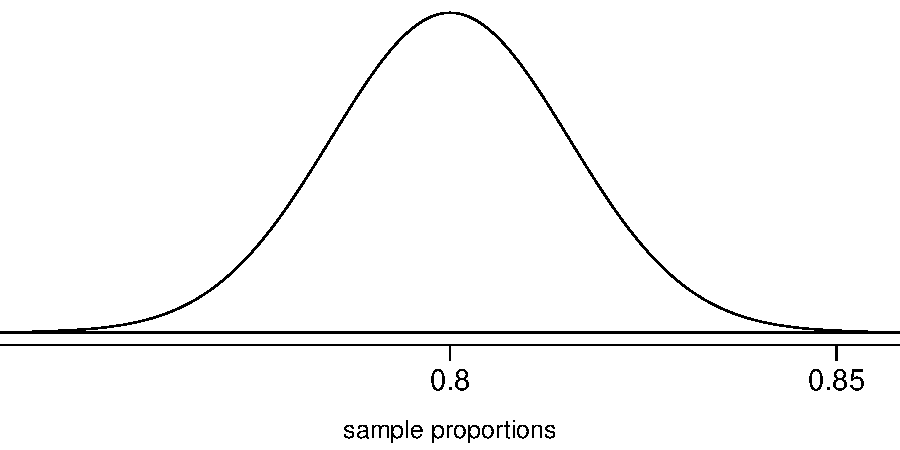
\includegraphics[width=\textwidth]{6-1_single_prop/expdesgn_norm.pdf}
\end{center}
}
\end{frame}
%%%%%%%%%%%%%%%%%%%%%%%%%%%%%%%%%%%

\begin{frame}
\frametitle{Prática}

\justifying
Como o o-valor é baixo, rejeitamos $H_0$. Os dados fornecem evidências convincentes de que mais de 80\% dos americanos têm uma boa intuição sobre desenho de experimentos.

\end{frame}

%%%%%%%%%%%%%%%%%%%%%%%%%%%%%%%%%%%

\subsection{Recapitulando}

%%%%%%%%%%%%%%%%%%%%%%%%%%%%%%%%%%%

\begin{frame}
\frametitle{Prática}

\pq{Em uma pesquisa do Gallup de 2006, 11\% de 1.001 americanos afirmaram que possuem resistência para celebrar o Halloween por motivos religiosos. Ao nível de confiança de 95\%, a margem de erro dessa pesquisa é de $\pm 3\%$. \\
Uma notícia, ao descobrir o resultado dessa pesquisa, publicou: "Mais de 10\% de todos os americanos possuem resistência para celebrar o Halloween por motivos religiosos". \\ Ao nível de confiança de 95\%, a declaração feita nessa notícia é justificada?}

\begin{enumerate}[(a)]
\item Sim
\solnMult{Não}
\item Nao sabe
\end{enumerate}

\end{frame}

%%%%%%%%%%%%%%%%%%%%%%%%%%%%%%%%%%

\begin{frame}
\frametitle{Recapitulando - inferência para uma proporção}

\begin{itemize}

\item Parâmetro da população: $p$, estimativa pontual: $\hat{p}$

\pause

\item Condições:
\begin{itemize}
\item independência \\
- amostra aleatória e condição 10\%
\item pelo menos 10 sucessos e fracassos\\ - se não $\rightarrow$ aleatorizar
\end{itemize}

\pause

\item Desvio Padrão: $SE = \sqrt{ \frac{p(1-p)}{n} }$
\begin{itemize}
\item para IC: usar $\hat{p}$
\item para TH: usar $p_0$
\end{itemize}

\end{itemize}

\end{frame}


%%%%%%%%%%%%%%%%%%%%%%%%%%%%%%%%%%%%

\section{6.2. Diferença entre proporções}

%%%%%%%%%%%%%%%%%%%%%%%%%%%%%%%%%%%%

\begin{frame}
\frametitle{Derretimento de calota de gelo}
\justifying
\pq{Cientistas preveem que o aquecimento global pode ter grandes consequências nas regiões polares nos próximos 100 anos. Um dos possíveis efeitos é que a calota de gelo do polo norte pode derreter completamente. Se isso acontecesse realmente, te incomodaria muito, um pouco, quase nada ou nada?}

\begin{enumerate}[(a)]
\item Muito
\item Um pouco
\item Quase nada
\item Nada
\end{enumerate}

\end{frame}

%%%%%%%%%%%%%%%%%%%%%%%%%%%%%%%%%%%

\begin{frame}
\frametitle{Resultados de uma pesquisa}
\justifying
Uma pesquisa americana faz a mesma pergunta e abaixo estão as distribuições de respostas. Além disso, essa mesma pergunta foi feita para um grupo de estudantes de estatística introdutória da Universidade de Duke: \\

\begin{center}
\begin{tabular}{l r r}
\hline
				& Pesquisa EUA	& Duke \\
\hline
Muito		& 454	& 69 \\
Um pouco			& 124 	& 30\\
Quase nada			& 52 		& 4\\
Nada			& 50 		& 2 \\
\hline
Total				& 680 	& 105\\
\hline
\end{tabular}
\end{center}

\end{frame}

%%%%%%%%%%%%%%%%%%%%%%%%%%%%%%%%%%

\begin{frame}
\frametitle{Estimativa paramétrica e pontual}

\begin{itemize}
\justifying
\item \hl{Parâmetro de interesse:} Diferença entre as proporções de \orange{todos} os alunos da Duke e \orange{todos} os americanos que ficariam muito incomodados com a calota de gelo do polo norte derretendo completamente.
\[ \mathhl{ p_{Duke} - p_{EUA} }\]

\pause

\justifying
\item \hl{Estimação pontual:} Diferença entre as proporções da \orange {amostra} de estudantes da Duke e da \orange {amostra} de americanos que ficariam muito incomodados com a calota de gelo do polo norte derretendo completamente.
\[ \mathhl{ \hat{p}_{Duke} - \hat{p}_{EUA} }\]

\end{itemize}

\end{frame}

%%%%%%%%%%%%%%%%%%%%%%%%%%%%%%%%%%%

\begin{frame}
\frametitle{Inferência para comparar proporções}

\begin{itemize}
\justifying
\item Os detalhes são os mesmos de antes...

\pause
\justifying
\item IC: \textcolor{orange}{$estimativa~pontual \pm margem~de~erro$}

\pause
\justifying
\item TH: Usar \textcolor{orange}{$Z = \frac{estimativa~pontual - valor~nulo}{SE}$} para encontrar o p-valor apropriado.

\pause
\justifying
\item Nós só precisamos do desvio padrão apropriado da estimativa pontual ($SE_{ \hat{p}_{Duke} - \hat{p}_{EUA}}$), que é o único novo conceito apresentado aqui.

\end{itemize}

\pause
\justifying
\formula{Desvio padrão da diferença entre duas proporções da amostra}
{
\[ SE_{(\hat{p}_1 - \hat{p}_2)} = \sqrt{ \frac{p_1(1-p_1)}{n_1} + \frac{p_2(1-p_2)}{n_2} } \]
}

\end{frame}

%%%%%%%%%%%%%%%%%%%%%%%%%%%%%%%%%%%%%

\subsection{Intervalos de confiança para diferença de proporções}

%%%%%%%%%%%%%%%%%%%%%%%%%%%%%%%%%%%%%

\begin{frame}
\frametitle{Condições para IC para diferença de proporções}

\begin{enumerate}
\justifying
\item \hl{Independência dentro dos grupos: }
\begin{itemize}
\justifying
\item O grupo dos EUA é amostrado aleatoriamente e estamos assumindo que o grupo Duke representa uma amostra aleatória também.
\pause
\justifying
\item $n_{Duke}$ $<$ 10\% de todos os alunos da Duke e 680 $ <$ 10 \% de todos os americanos.
\end{itemize}
\pause
\justifying
Podemos supor que as respostas dos alunos da Duke na amostra são independentes umas das outras, e as respostas dos americanos na amostra são independentes umas das outras também.

\pause
\justifying
\item \hl{Independência entre grupos: }
Os alunos amostrados da Duke e os americanos na pesquisa EUA são independentes uns dos outros.

\pause
\justifying
\item \hl{Sucesso-falha:} 
Pelo menos 10 sucessos observados e 10 falhas observadas nos dois grupos.

\end{enumerate}

\end{frame}

%%%%%%%%%%%%%%%%%%%%%%%%%%%%%%%%%%%%%

\begin{frame}
\frametitle{Prática}
\justifying
\dq{Construa um intervalo de confiança de 95\% para a diferença entre as proporções de alunos da Duke e de americanos que seriam muito incomodados com o derretimento da calota de gelo do polo norte \orange{($p_{Duke} - p_{EUA}$)}.}

{\footnotesize
\begin{center}
\begin{tabular}{l | c c}
Dados			& Duke		& EUA \\
\hline
Muito	& 69			& 454 \\
Nada & 36			& 226 \\
\hline
Total			& 105		& 680 \\
\hline
\pause
$\hat{p}$		& 0.657		& 0.668
\end{tabular}
\end{center}
}

\end{frame}
%%%%%%%%%%%%%%%%%%%%%%%%%%%%%%%%%%%%%

\begin{frame}
\frametitle{Prática}

\soln{
\begin{eqnarray*}
&& (\hat{p}_{Duke} - \hat{p}_{EUA}) \pm z^\star \times \sqrt{ \frac{ \hat{p}_{Duke} (1 - \hat{p}_{Duke})}{n_{Duke} } + \frac{ \hat{p}_{EUA} (1 -  \hat{p}_{EUA})}{n_{EUA} } }  \\
\pause
&=& (0.657 - 0.668) \pause \pm 1.96 \pause \times \sqrt{ \frac{0.657 \times 0.343}{105} + \frac{0.668 \times 0.332}{680} } \\
\pause
&=& -0.011 \pm \pause 1.96 \times 0.0497 \\
\pause
&=& -0.011 \pm 0.097 \\
\pause
&=& (-0.108, 0.086)
\end{eqnarray*}
}


\end{frame}

%%%%%%%%%%%%%%%%%%%%%%%%%%%%%%%%%%%%%

\subsection{HT para comparar proporções}

%%%%%%%%%%%%%%%%%%%%%%%%%%%%%%%%%%%%%

\begin{frame}
\frametitle{Prática}
\justifying
\pq{Qual dos seguintes conjuntos de hipóteses é o correto para testar se a proporção de pessoas que ficariam muito incomodados pelo derretimento da calota de gelo do polo norte entre os alunos da Duke difere da proporção de todos os americanos que também ficariam muito incomodados?}

\begin{enumerate}[(a)]
\solnMult{ $H_0:  p_{Duke} = p_{EUA}$ \\
$H_A:  p_{Duke} \ne p_{US}$ }
\item $H_0:  \hat{p}_{Duke} = \hat{p}_{EUA}$ \\
$H_A:  \hat{p}_{Duke} \ne \hat{p}_{EUA}$
\solnMult{ $H_0:  p_{Duke} - p_{EUA} = 0$ \\
$H_A:  p_{Duke} - p_{EUA} \ne 0$ }
\item $H_0:  p_{Duke} = p_{EUA}$ \\
$H_A:  p_{Duke} < p_{EUA}$
\end{enumerate}

\soln{
\only<2>{\orange{Ambos (a) e (c) estão corretas.}}
}

\end{frame}

%%%%%%%%%%%%%%%%%%%%%%%%%%%%%%%%%%

\begin{frame}
\frametitle{Flashback para trabalhar com uma proporção}

\begin{itemize}
\justifying
\item Ao construir um intervalo de confiança para uma proporção da população, verificamos se o número de sucessos e falhas \orange {observado} é pelo menos 10.
\[ n\hat{p} \ge 10 \qquad \qquad n(1-\hat{p}) \ge 10 \]

\pause
\justifying
\item Ao conduzir um teste de hipótese para uma proporção da população, verificamos se o número de sucessos e falhas \orange {esperado} é de pelo menos 10.
\[ np_0 \ge 10 \qquad \qquad n(1-p_0) \ge 10 \]

\end{itemize}

\end{frame}

%%%%%%%%%%%%%%%%%%%%%%%%%%%%%%%%%%%

\begin{frame}
\frametitle{Estimativa agrupada de uma proporção}

\begin{itemize}
\justifying
\item No caso de comparar duas proporções onde $ H_0: p_1 = p_2 $, não há um valor nulo que possamos usar para calcular o número de sucessos e falhas \orange {esperado} em cada amostra.

\pause
\justifying
\item Portanto, precisamos primeiro encontrar uma proporção comum (\hl {agrupado}) para os dois grupos e usá-la em nossa análise.

\pause
\justifying
\item Isso significa encontrar a proporção de sucessos totais entre o número total de observações.

\end{itemize}

$\:$ \\
\justifying
\formula{Estimativa agrupada de uma proporção}
{ \[ \hat{p} = \frac{\#~de~sucessos_1 + \#~de~sucessos_2}{n_1 + n_2} \] }

\end{frame}

%%%%%%%%%%%%%%%%%%%%%%%%%%%%%%%%%%%

\begin{frame}
\frametitle{Prática}
\justifying
\dq{Calcular a estimativa \underline{proporção combinada} de estudantes da Duke e americanos que se incomodariam muito com o derretimento da calota de gelo do polo norte. De qual proporção amostrada ($\hat{p}_{Duke}$ ou $\hat{p}_{EUA}$) a estimativa agrupada está mais próxima? Por quê?}

{\footnotesize
\begin{center}
\begin{tabular}{l | c c}
Data			& Duke		& EUA \\
\hline
Muito	& 69			& 454 \\
Nada & 36			& 226 \\
\hline
Total			& 105		& 680 \\
\hline
$\hat{p}$		& 0.657		& 0.668
\end{tabular}
\end{center}
}

\pause

\soln{
\begin{eqnarray*}
\hat{p} &=& \frac{\#~de~sucessos_1 + \#~de~sucessos_2}{n_1 + n_2} \\
\pause
&=& \frac{69+454}{105+680} \pause = \frac{523}{785} \pause = 0.666
\end{eqnarray*}
}

\end{frame}
%%%%%%%%%%%%%%%%%%%%%%%%%%%%%%%%%%%

\begin{frame}
\frametitle{Prática}
\justifying
\dq{Esses dados sugerem que a proporção de todos os alunos da Duke que seriam muito incomodados pelo derretimento da calota de gelo do norte difere da proporção de todos os americanos que o fazem? Calcule a estatística de teste, o valor p e interprete sua conclusão no contexto dos dados.}

{\footnotesize
\begin{center}
\begin{tabular}{l | c c}
Dados			& Duke		& US \\
\hline
Muito	& 69			& 454 \\
Nada & 36			& 226 \\
\hline
Total			& 105		& 680 \\
\hline
$\hat{p}$		& 0.657		& 0.668
\end{tabular}
\end{center}
}

\pause
\end{frame}
%%%%%%%%%%%%%%%%%%%%%%%%%%%%%%%%%%%

\begin{frame}
\frametitle{Prática}

\soln{
\begin{eqnarray*}
Z &=& \frac{(\hat{p}_{Duke} - \hat{p}_{EUA})}{\sqrt{ \frac{ \hat{p} (1 - \hat{p})}{n_{Duke} } + \frac{ \hat{p} (1 -  \hat{p})}{n_{EUA} } }} \\
\pause 
&=& \frac{(0.657 - 0.668)}{\sqrt{ \frac{0.666 \times 0.334}{105} + \frac{0.666 \times 0.334}{680} }} = \pause \frac{-0.011}{0.0495} \pause = -0.22 \\
\pause
p-valor &=& 2 \times P(Z < -0.22) \pause = 2 \times 0.41 = 0.82
\end{eqnarray*}
}

\end{frame}

%%%%%%%%%%%%%%%%%%%%%%%%%%%%%%%%%%%

\subsection{Recapitular}

%%%%%%%%%%%%%%%%%%%%%%%%%%%%%%%%%%%

\begin{frame}
\frametitle{Recapitulação - comparando duas proporções}

\begin{itemize}
\justifying
\item Parâmetro de população: $(p_1 - p_2)$, estimativa pontual: $(\hat{p}_1 - \hat{p}_2)$

\pause

\item Condições:
\pause
\begin{itemize}
\justifying
\item independência dentro dos grupos \\
\justifying
- amostra aleatória e condição de 10\% atendidas para ambos os grupos
\justifying
\item independência entre grupos
\justifying
\item pelo menos 10 sucessos e falhas em cada grupo\\ 
\justifying
- se não $\rightarrow$ aleatorizar (Seção 6.4)
\end{itemize}

\pause
\justifying
\item $SE_{(\hat{p}_1 - \hat{p}_2)} = \sqrt{ \frac{p_1(1-p_1)}{n_1} + \frac{p_2(1-p_2)}{n_2} }$
\begin{itemize}
\justifying
\item para IC: usar $\hat{p}_1$ e $\hat{p}_2$
\justifying
\item para TH:
\begin{itemize}
\justifying
\item quando $H_0: p_1 = p_2$: usar $\hat{p}_{agrupado} = \frac{\#~suc_1 + \#suc_2}{n_1 + n_2}$
\justifying
\item quando $H_0: p_1 - p_2 = $ \textit{(algum valor diferente de 0)}: usar $\hat{p}_1$ e $\hat{p}_2$ \\
- isso é muito raro
\end{itemize}
\end{itemize}

\end{itemize}

\end{frame}

%%%%%%%%%%%%%%%%%%%%%%%%%%%%%%%%%%%

\begin{frame}
\frametitle{Referência - cálculos de erro padrão}

\begin{center}
\begin{tabular}{l | l | l}
			& uma amostra					& duas amostras \\ 
\hline
& & \\
média		& $SE = \frac{s}{\sqrt{n}}$			& $SE = \sqrt{ \frac{s_1^2}{n_1} + \frac{s_2^2}{n_2}}$ \\
& & \\
\hline
& & \\
proporção		& $SE = \sqrt{ \frac{p(1-p)}{n} }$	& $SE = \sqrt{ \frac{p_1(1-p_1)}{n_1} + \frac{p_2(1-p_2)}{n_2} }$	 \\	
& & \\
\end{tabular}
\end{center}

\pause

\begin{itemize}
\justifying
\item Ao trabalhar com médias, é muito raro que $\sigma$ seja conhecido, então geralmente usamos $s$.

\pause
\justifying
\item Ao trabalhar com proporções, 
\begin{itemize}
\justifying
\item se fazemos um teste de hipótese, $p$ vem da hipótese nula
\justifying
\item se construimos um intervalo de confiança, use $\hat{p}$
\end{itemize}

\end{itemize}

\end{frame}
%%%%%%%%%%%%%%%%%%%%%%%%%%%%%%%%%%%%

\section{6.3. Teste qui-quadrado de \textit{Goodness of fit}}

%%%%%%%%%%%%%%%%%%%%%%%%%%%%%%%%%%%

\subsection{Dados de Weldon}

%%%%%%%%%%%%%%%%%%%%%%%%%%%%%%%%%%%

\begin{frame}
\frametitle{Dados de Weldon}

\twocol{0.7}{0.3}
{
\begin{itemize}
\justifying
\small
\item Walter Frank Raphael Weldon (1860 - 1906), foi um biólogo inglês evolucionário e um dos fundadores da biometria. Além disso, ele foi o editor fundador da revista \textit{Biometrika}, com Francis Galton e Karl Pearson.
\justifying
\item Em 1894, ele jogou 12 dados 26.306 vezes e registrou a quatidade de vezes que sairam os número 5 e 6 (que ele considerou como sucesso).

\end{itemize}
}
{
\begin{center}
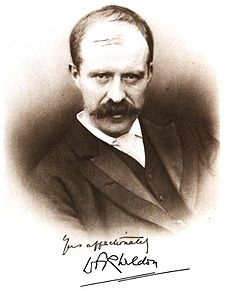
\includegraphics[width=\textwidth]{6-3_chisq_gof/weldon.jpeg}
\end{center}
}
\begin{itemize}
\justifying
\small
\item Observou-se que os números 5 ou 6 ocorreram com mais frequência do que o esperado, e Pearson levantou a hipótese de que isso ocorreu provavelmente devido à construção dos dados. Os dados mais baratos têm pips (aqueles pontinhos pretos) ocos e, como os lados opostos aumentam para 7, a face com 6 pips é mais leve do que a face oposta, que tem apenas 1 pip.

\end{itemize}

\end{frame}

%%%%%%%%%%%%%%%%%%%%%%%%%%%%%%%%%%%

\begin{frame}
\frametitle{Dados de Labby}
\scalefont{0.8}
\twocol{0.5}{0.5}
{
\begin{itemize}
\justifying
\item Em 2009, Zacariah Labby (U de Chicago), repetiu o experimento de Weldon usando uma máquina de contagem de lançadores de dados caseiros.
\begin{center}
\justifying
\webURL{http://www.youtube.com/watch?v=95EErdouO2w}
\end{center}
\justifying
\item O processo de criação de imagens demorava cerca de 20 segundos por rolagem.

\end{itemize}
}
{
\begin{center}
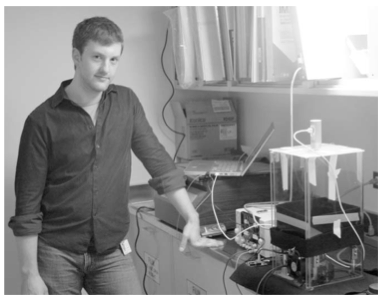
\includegraphics[width=\textwidth]{6-3_chisq_gof/labby.png}
\end{center}
}

\begin{itemize}
\justifying
\item Cada dia havia $\sim$ 150 imagens para processar manualmente.
\justifying
\item Nesse ritmo, a experiência de Weldon foi repetida em pouco mais de seis dias inteiros.
\justifying
\item Leitura recomendada:\webURL{http://galton.uchicago.edu/about/docs/labby09dice.pdf}

\end{itemize}

\end{frame}

%%%%%%%%%%%%%%%%%%%%%%%%%%%%%%%%%%%

\begin{frame}
\frametitle{Dados de Labby (cont.)}

\begin{itemize}
\justifying
\item Labby não observou o mesmo fenômeno que Weldon (maior frequência dos números de 5 e 6).
\justifying
\item A automação permitiu que Labby coletasse mais dados do que Weldon em 1894, e, em vez de registrar "sucessos" e "falhas", Labby registrava o número individual de pips em cada dado.

\end{itemize}

\begin{center}
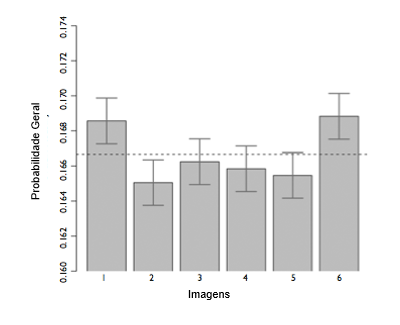
\includegraphics[width=0.5\textwidth]{6-3_chisq_gof/labbyPipCounts.png}
\end{center}

\end{frame}

%%%%%%%%%%%%%%%%%%%%%%%%%%%%%%%%%%%

\subsection*{Criando uma estatística de teste para tabelas unidirecionais}

%%%%%%%%%%%%%%%%%%%%%%%%%%%%%%%%%%%

\begin{frame}
\frametitle{Contagens esperadas}
\justifying
\pq{Labby rolou 12 dados 26.306 vezes. Se cada lado tiver a mesma probabilidade de aparecer, quantos 1s, 2s, $\cdots$, 6s ele esperaria observar?}

\begin{enumerate}[(a)]
\item $\frac{1}{6}$
\item $\frac{12}{6}$
\item $\frac{26,306}{6}$
\solnMult{ $\frac{12 \times 26,306}{6}$ } \soln{\only<2>{\orange{$= 52,612$}}}
\end{enumerate}

\end{frame}

%%%%%%%%%%%%%%%%%%%%%%%%%%%%%%%%%%%

\begin{frame}
\frametitle{Sumarizando os resultados de Labby}
\justifying
A tabela abaixo mostra as contagens observadas e esperadas da experiência de Labby.

{
\begin{center}
\renewcommand\arraystretch{1.25}
\scalefont{0.7}
\begin{tabular}{c | c c}
Resultado	& Observado	& Esperado \\
\hline
1		& 53,222		& 52,612 \\
2		& 52,118		& 52,612 \\
3		& 52,465		& 52,612 \\
4		& 52,338		& 52,612 \\
5		& 52,244		& 52,612 \\
6		& 53,285		& 52,612 \\
\hline
Total		& 315,672		& 315,672
\end{tabular}
\end{center}
}

\pause
\small{\justifying
\dq{Por que, para todos os resultados, as contagens esperadas são as mesmas mas as contagens observadas são diferentes? À primeira vista, parece haver uma inconsistência entre as contagens observadas e esperadas?}
}
\end{frame}

%%%%%%%%%%%%%%%%%%%%%%%%%%%%%%%%%%%

\begin{frame}
\frametitle{Definindo as hipóteses}
\justifying
\dq{Esses dados fornecem evidências convincentes de uma inconsistência entre as contagens observadas e esperadas?}

\pause

\begin{itemize}
\justifying
\item[$H_0$:] Não há inconsistência entre as contagens observadas e as esperadas. \hlGr{As contagens observadas seguem a mesma distribuição que as contagens esperadas.}

\pause
\justifying
\item[$H_A$:] Existe uma inconsistência entre as contagens observadas e as esperadas. \hlGr{As contagens observadas \orange {não} seguem a mesma distribuição das contagens esperadas.} Existe um viés para que um lado apareça mais vezes no lançamento de um dado.
\end{itemize}

\end{frame}

%%%%%%%%%%%%%%%%%%%%%%%%%%%%%%%%%%%

\begin{frame}
\frametitle{Avaliando as hipóteses}

\begin{itemize}
\justifying
\item Para avaliar essas hipóteses, quantificamos quão diferentes são as contagens observadas das contagens esperadas.

\pause
\justifying
\item Grandes desvios do que seria esperado com base na variação amostral por si só fornecem fortes evidências para a hipótese alternativa.

\pause
\justifying
\item Isso é chamado de teste de \hl{goodness of fit}, ou \textit{qualidade de ajuste}, pois estamos avaliando o quão bem os dados observados se ajustam à distribuição esperada.

\end{itemize}

\end{frame}

%%%%%%%%%%%%%%%%%%%%%%%%%%%%%%%%%%%

\subsection{A estatística do teste do qui-quadrado}

%%%%%%%%%%%%%%%%%%%%%%%%%%%%%%%%%%%

\begin{frame}
\frametitle{Anatomia de uma estatística de teste}

\begin{itemize}
\justifying
\item A forma geral de uma estatística de teste é
\[ \frac{\text{estimativa pontual} - \text{valor nulo}}{\text{erro padrão da estimativa pontual}} \]

\pause
\justifying
\item Esta construção é baseada em 
\begin{enumerate}
\justifying
\item identificar a diferença entre uma estimativa pontual e um valor esperado, supondo que a hipótese nula é verdadeira, e
\justifying
\item padronizar essa diferença usando o erro padrão da estimativa pontual. 
\end{enumerate}
\pause
\justifying
Essas duas ideias ajudarão na construção de uma estatística de teste apropriada para dados de contagem.

\end{itemize}

\end{frame}

%%%%%%%%%%%%%%%%%%%%%%%%%%%%%%%%%%%

\begin{frame}
\frametitle{Estatística qui-quadrado}
\justifying
Ao lidar com contagens e investigar quão longe as contagens observadas estão das contagens esperadas, usamos uma nova estatística de teste chamada \hl{estatística de qui-quadrado ($ \chi^2 $)}.

$\:$ \\

\pause

\formula{Estatística de $\chi^2$ }
{
\[\chi^2 = \sum_{i = 1}^k \frac{(O - E)^2}{E} \qquad \text{onde $k$ = número total de células} \]
}

\end{frame}

%%%%%%%%%%%%%%%%%%%%%%%%%%%%%%%%%%%

\begin{frame}
\frametitle{Calculando a estatística do qui-quadrado}

\begin{center}
\renewcommand\arraystretch{1.8}
\begin{tabular}{c | c c | c}
Resultado	& Observado	& Esperado 	& $\frac{(O - E)^2}{E}$\\
\hline
1		& 53,222		& 52,612 		& $\frac{(53,222 - 52,612)^2}{52,612} = 7.07$ \\
\pause
2		& 52,118		& 52,612 		& $\frac{(52,118 - 52,612)^2}{52,612} = 4.64$ \\
\pause
3		& 52,465		& 52,612 		& $\frac{(52,465 - 52,612)^2}{52,612} = 0.41$ \\
\pause
4		& 52,338		& 52,612 		& $\frac{(52,338 - 52,612)^2}{52,612} = 1.43$\\
\pause
5		& 52,244		& 52,612 		& $\frac{(52,244 - 52,612)^2}{52,612} = 2.57$\\
\pause
6		& 53,285		& 52,612 		& $\frac{(53,285 - 52,612)^2}{52,612} = 8.61$\ \\
\hline
\pause
Total		& 315,672		& 315,672		& 24.73
\end{tabular}
\end{center}

\end{frame}

%%%%%%%%%%%%%%%%%%%%%%%%%%%%%%%%%%%

\begin{frame}
\frametitle{Por que qui-\underline{quadrado}?}

\justifying
Tomar o quadrado da diferença entre o resultado observado e o esperado permite duas coisas duas coisas:
\pause
\begin{itemize}
\justifying
\item Qualquer diferença padronizada que seja quadrada será agora positiva.
\pause
\justifying
\item Diferenças que já pareciam incomuns se tornarão muito maiores depois de se tomar o quadrado.
\end{itemize}

\vspace{1cm}

\pause
\justifying
\dq{Quando já vimos isso antes?}

\end{frame}

%%%%%%%%%%%%%%%%%%%%%%%%%%%%%%%%%%%

\subsection{A distribuição de qui-quadrado e áreas de descoberta}

%%%%%%%%%%%%%%%%%%%%%%%%%%%%%%%%%%%

\begin{frame}
\frametitle{A distribuição de qui-quadrado}

\begin{itemize}
\justifying
\item Para determinar se a estatística $\chi^2$ que calculamos é considerada excepcionalmente alta ou não, precisamos primeiro descrever sua distribuição.

\pause
\justifying
\item A distribuição qui-quadrado tem apenas um parâmetro chamado \hl {graus de liberdade (df)}, que influencia a forma, o centro e a largura da distribuição. \\

\end{itemize}

\pause

$\:$ \\
\justifying
\scalefont{0.8}
Lembre-se que até agora, vimos três outras distribuições contínuas:
\begin{itemize}
\justifying
\item[-] Distribuição normal: unimodal e simétrica com dois parâmetros (média e desvio padrão).
\justifying
\item[-] Distribuição T: unimodal e simétrica com um parâmetro (graus de liberdade).
\justifying
\item[-] Distribuição F: unimodal e inclinada à direita com dois parâmetros (graus de liberdade ou numerador, que é a variância entre grupos, e denominador, que é a varição dentro do grupo).
\end{itemize}


\end{frame}

%%%%%%%%%%%%%%%%%%%%%%%%%%%%%%%%%%%

\begin{frame}
\footnotesize
\frametitle{Prática}
\justifying
\pq{Qual das seguintes afirmações é falsa?}

\begin{center}
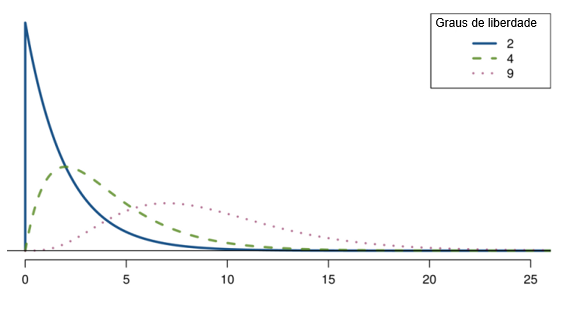
\includegraphics[width=0.7\textwidth]{6-3_chisq_gof/chiSquareDistributionWithInceasingDF.png}
\end{center}

À medida que df aumenta,
\begin{enumerate}[(a)]
\justifying
\item o centro da distribuição $\chi^2$ aumenta também.
\justifying
\item a variabilidade da distribuição $\chi^2$ aumenta também.
\justifying
\solnMult{a forma da distribuição $\chi^2$ torna-se mais assimétrica (menos parecida com uma normal).}
\end{enumerate}

\end{frame}

%%%%%%%%%%%%%%%%%%%%%%%%%%%%%%%%%%%

\begin{frame}[fragile]
\frametitle{Encontrando a área sob a curva da distribuição qui-quadrado}

\begin{itemize}
\justifying
\item P-valor = área da cauda sob a distribuição qui-quadrado.

\pause
\justifying
\item Para isso, podemos usar uma linguagem de programação, ou uma \hl{tabela de probabilidades qui-quadrado}.

\pause
\justifying
\item  Esta tabela funciona como a tabela $t$, mas fornece apenas os valores de cauda superiores.
\end{itemize}

\begin{center}
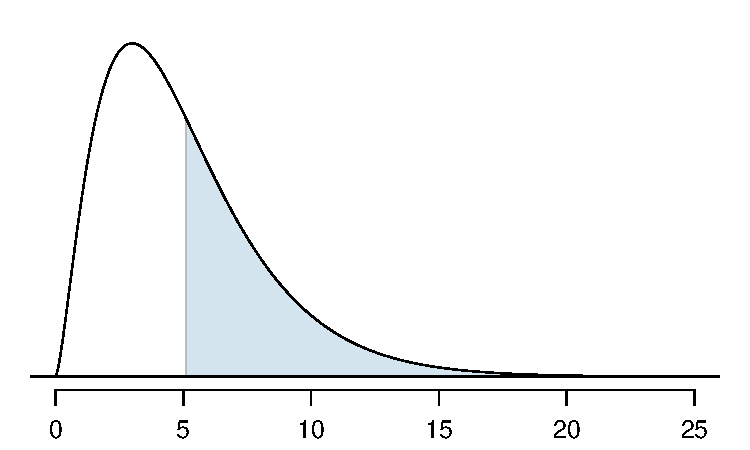
\includegraphics[width=0.6\textwidth]{6-3_chisq_gof/above5Point1WithDF5.pdf}
\end{center}

\end{frame}
%%%%%%%%%%%%%%%%%%%%%%%%%%%%%%%%%%%

\begin{frame}[fragile]
\frametitle{Encontrando a área sob a curva da distribuição qui-quadrado}

{\scriptsize
\begin{center}
\begin{tabular}{r | rrrr | rrrr |}
  \hline
Cauda superior & 0.3 & 0.2 & 0.1 & 0.05 & 0.02 & 0.01 & 0.005 & 0.001 \\ 
  \hline
df \hfill 1 &  1.07 &  1.64 &  2.71 &  3.84 &  5.41 &  6.63 &  7.88 &  10.83 \\ 
  2 &  2.41 &  3.22 &  4.61 &  5.99 &  7.82 &  9.21 &  10.60 &  13.82 \\ 
  3 &  3.66 &  4.64 &  6.25 &  7.81 &  9.84 &  11.34 &  12.84 &  16.27 \\ 
  4 &  4.88 &  5.99 &  7.78 &  9.49 &  11.67 &  13.28 &  14.86 &  18.47 \\ 
  5 &  6.06 &  7.29 &  9.24 &  11.07 &  13.39 &  15.09 &  16.75 &  20.52 \\ 
  \hline
  6 &  7.23 &  8.56 &  10.64 &  12.59 &  15.03 &  16.81 &  18.55 &  22.46 \\ 
  7 &  8.38 &  9.80 &  12.02 &  14.07 &  16.62 &  18.48 &  20.28 &  24.32 \\ 
  $\cdots$ &   &   &   &   &   &   &   &   \\ 
\end{tabular}
\end{center}
}

\end{frame}

%%%%%%%%%%%%%%%%%%%%%%%%%%%%%%%%%%%

\begin{frame}
\frametitle{Encontrando a área sob a curva da distribuição qui-quadrado}
\justifying
\dq{Estimar a área sombreada sob a curva da distribuição qui-quadrado com $df = 6$.}

\twocol{0.6}{0.4}{
\begin{center}
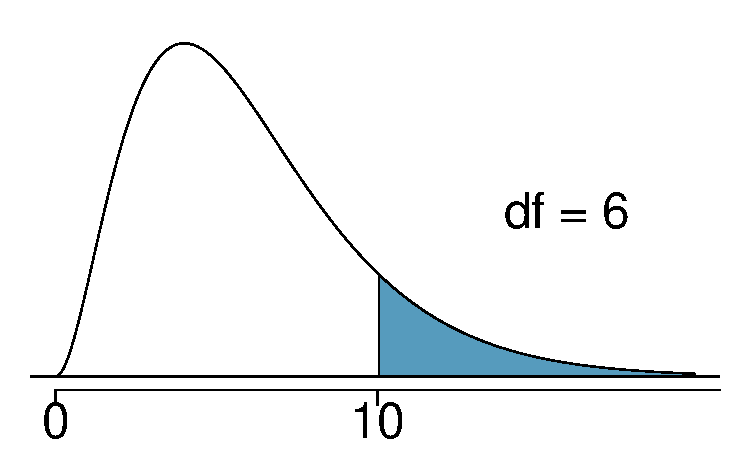
\includegraphics[width=0.67\textwidth]{6-3_chisq_gof/above10WithDF6.pdf}
\end{center}
}
{\only<2 |handout:0>{\orange{$P(\chi^2_{df = 6} > 10)$\\ está entre 0.1 e 0.2}}
}
\end{frame}
%%%%%%%%%%%%%%%%%%%%%%%%%%%%%%%%%%%

\begin{frame}
\frametitle{Encontrando a área sob a curva da distribuição qui-quadrado}

\only<1>{
\begin{center}
{\footnotesize
\begin{tabular}{r | rrrr | rrrr |}
  \hline
Cauda superior & 0.3 & 0.2 & 0.1 & 0.05 & 0.02 & 0.01 & 0.005 & 0.001 \\ 
  \hline
df \hfill 1 &  1.07 &  1.64 &  2.71 &  3.84 &  5.41 &  6.63 &  7.88 &  10.83 \\ 
  2 &  2.41 &  3.22 &  4.61 &  5.99 &  7.82 &  9.21 &  10.60 &  13.82 \\ 
  3 &  3.66 &  4.64 &  6.25 &  7.81 &  9.84 &  11.34 &  12.84 &  16.27 \\ 
  4 &  4.88 &  5.99 &  7.78 &  9.49 &  11.67 &  13.28 &  14.86 &  18.47 \\ 
  5 &  6.06 &  7.29 &  9.24 &  11.07 &  13.39 &  15.09 &  16.75 &  20.52 \\ 
  \hline
  6 &  7.23 &  8.56 &   10.64  &  12.59 &  15.03 &  16.81 &  18.55 &  22.46 \\ 
  7 &  8.38 &  9.80 &  12.02 &  14.07 &  16.62 &  18.48 &  20.28 &  24.32 \\ 
  \hline
\end{tabular}
}
\end{center}
}

\only<2 | handout:0>{
\begin{center}
{\footnotesize
\begin{tabular}{r | rrrr | rrrr |}
  \hline
Cauda superior & 0.3 & 0.2 & 0.1 & 0.05 & 0.02 & 0.01 & 0.005 & 0.001 \\ 
  \hline
df \hfill 1 &  1.07 &  1.64 &  2.71 &  3.84 &  5.41 &  6.63 &  7.88 &  10.83 \\ 
  2 &  2.41 &  3.22 &  4.61 &  5.99 &  7.82 &  9.21 &  10.60 &  13.82 \\ 
  3 &  3.66 &  4.64 &  6.25 &  7.81 &  9.84 &  11.34 &  12.84 &  16.27 \\ 
  4 &  4.88 &  5.99 &  7.78 &  9.49 &  11.67 &  13.28 &  14.86 &  18.47 \\ 
  5 &  6.06 &  7.29 &  9.24 &  11.07 &  13.39 &  15.09 &  16.75 &  20.52 \\ 
  \hline
\rowcolor[gray]{.6}
  6 &  7.23 &  8.56 &   10.64  &  12.59 &  15.03 &  16.81 &  18.55 &  22.46 \\ 
  7 &  8.38 &  9.80 &  12.02 &  14.07 &  16.62 &  18.48 &  20.28 &  24.32 \\ 
  \hline
\end{tabular}
}
\end{center}
}

\only<3 | handout:0>{
\begin{center}
{\footnotesize
\begin{tabular}{r | rrrr | rrrr |}
  \hline
Cauda superior & 0.3 & 0.2 & 0.1 & 0.05 & 0.02 & 0.01 & 0.005 & 0.001 \\ 
  \hline
df \hfill 1 &  1.07 &  1.64 &  2.71 &  3.84 &  5.41 &  6.63 &  7.88 &  10.83 \\ 
  2 &  2.41 &  3.22 &  4.61 &  5.99 &  7.82 &  9.21 &  10.60 &  13.82 \\ 
  3 &  3.66 &  4.64 &  6.25 &  7.81 &  9.84 &  11.34 &  12.84 &  16.27 \\ 
  4 &  4.88 &  5.99 &  7.78 &  9.49 &  11.67 &  13.28 &  14.86 &  18.47 \\ 
  5 &  6.06 &  7.29 &  9.24 &  11.07 &  13.39 &  15.09 &  16.75 &  20.52 \\ 
  \hline
  \rowcolor[gray]{.6}
  6 &  7.23 & \orange{ 8.56 }&  \orange{ 10.64 } &  12.59 &  15.03 &  16.81 &  18.55 &  22.46 \\ 
  7 &  8.38 &  9.80 &  12.02 &  14.07 &  16.62 &  18.48 &  20.28 &  24.32 \\ 
  \hline
\end{tabular}
}
\end{center}
}

\only<4 | handout:0>{
\begin{center}
{\footnotesize
\begin{tabular}{r | r >{\columncolor[gray]{0.6}[.5\tabcolsep]}r >{\columncolor[gray]{0.6}[.5\tabcolsep]}rr | rrrr |}
  \hline
Cauda superior & 0.3 & \orange{0.2} & \orange{0.1} & 0.05 & 0.02 & 0.01 & 0.005 & 0.001 \\ 
  \hline
df \hfill 1 &  1.07 &  1.64 &  2.71 &  3.84 &  5.41 &  6.63 &  7.88 &  10.83 \\ 
  2 &  2.41 &  3.22 &  4.61 &  5.99 &  7.82 &  9.21 &  10.60 &  13.82 \\ 
  3 &  3.66 &  4.64 &  6.25 &  7.81 &  9.84 &  11.34 &  12.84 &  16.27 \\ 
  4 &  4.88 &  5.99 &  7.78 &  9.49 &  11.67 &  13.28 &  14.86 &  18.47 \\ 
  5 &  6.06 &  7.29 &  9.24 &  11.07 &  13.39 &  15.09 &  16.75 &  20.52 \\ 
  \hline
  \rowcolor[gray]{.6}
  6 &  7.23 & \orange{ 8.56 }&  \orange{ 10.64 } &  12.59 &  15.03 &  16.81 &  18.55 &  22.46 \\ 
  7 &  8.38 &  9.80 &  12.02 &  14.07 &  16.62 &  18.48 &  20.28 &  24.32 \\ 
  \hline
\end{tabular}
}
\end{center}
}

\end{frame}

%%%%%%%%%%%%%%%%%%%%%%%%%%%%%%%%%%%

\begin{frame}
\frametitle{Encontrando a área sob a curva da distribuição qui-quadrado}
\justifying
\pq{Estime a área sombreada (acima de 17) sob a curva $ \chi ^ 2 $ com $df = 9$.}

\twocol{0.6}{0.4}{
\begin{center}
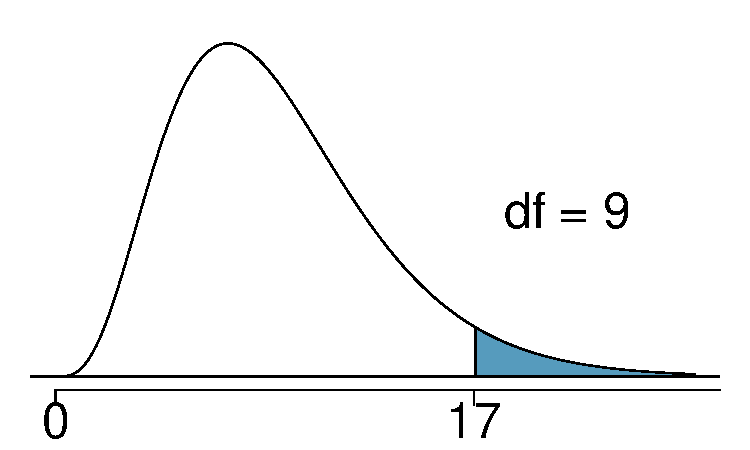
\includegraphics[width=0.67\textwidth]{6-3_chisq_gof/above17WithDF9.pdf}
\end{center}
}
{
{\small
\begin{enumerate}[(a)]
\setlength{\itemsep}{0in}
\item 0.05
\item 0.02
\solnMult{entre 0.02 e 0.05}
\item entre 0.05 e 0.1
\item entre 0.01 e 0.02
\end{enumerate}
}
}
\end{frame}
%%%%%%%%%%%%%%%%%%%%%%%%%%%%%%%%%%%

\begin{frame}
\frametitle{Encontrando a área sob a curva da distribuição qui-quadrado}

\only<1>{
\begin{center}
{\scriptsize
\begin{tabular}{r | rrrr | rrrr |}
  \hline
Cauda superior & 0.3 & 0.2 & 0.1 & 0.05 & 0.02 & 0.01 & 0.005 & 0.001 \\ 
  \hline
df  \hfill 7 &  8.38 &  9.80 &  12.02 &  14.07 &  16.62 &  18.48 &  20.28 &  24.32 \\ 
  8 &  9.52 &  11.03 &  13.36 &  15.51 &  18.17 &  20.09 &  21.95 &  26.12 \\ 
  9 &  10.66 &  12.24 &  14.68 &  16.92 &  19.68 &  21.67 &  23.59 &  27.88 \\ 
  10 &  11.78 &  13.44 &  15.99 &  18.31 &  21.16 &  23.21 &  25.19 &  29.59 \\ 
  \hline
  11 &   12.90 &  14.63 &  17.28 &  19.68 &  22.62 &  24.72 &  26.76 &  31.26 \\ 
\end{tabular}
}
\end{center}
}

\only<2 | handout:0>{
\begin{center}
{\scriptsize
\begin{tabular}{r | rrr >{\columncolor[gray]{0.6}[.5\tabcolsep]}r | >{\columncolor[gray]{0.6}[.5\tabcolsep]}rrrr |}
  \hline
Cauda superior & 0.3 & 0.2 & 0.1 & \orange{ 0.05 } & \orange{ 0.02 } & 0.01 & 0.005 & 0.001 \\ 
  \hline
df  \hfill 7 &  8.38 &  9.80 &  12.02 &  14.07 &  16.62 &  18.48 &  20.28 &  24.32 \\ 
  8 &  9.52 &  11.03 &  13.36 &  15.51 &  18.17 &  20.09 &  21.95 &  26.12 \\ 
    \rowcolor[gray]{.6}
  9 &  10.66 &  12.24 &  14.68 &  \orange{16.92 }&  \orange{19.68} &  21.67 &  23.59 &  27.88 \\ 
  10 &  11.78 &  13.44 &  15.99 &  18.31 &  21.16 &  23.21 &  25.19 &  29.59 \\ 
  \hline
  11 &   12.90 &  14.63 &  17.28 &  19.68 &  22.62 &  24.72 &  26.76 &  31.26 \\ 
  \hline
\end{tabular}
}
\end{center}
}

\end{frame}

%%%%%%%%%%%%%%%%%%%%%%%%%%%%%%%%%%%

\begin{frame}
\frametitle{Encontrando a área sob a curva da distribuição qui-quadrado}
\justifying
\pq{Estime a área sombreada (acima de 30) sob a curva $ \chi ^ 2 $ com $df = 10$.}

\twocol{0.6}{0.4}{
\begin{center}
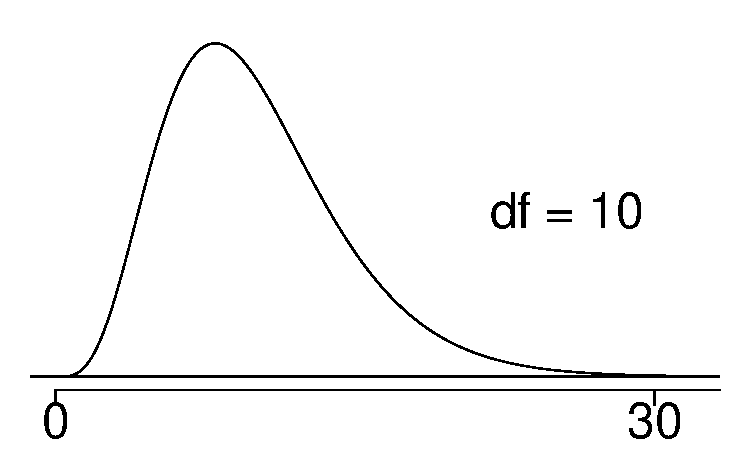
\includegraphics[width=0.67\textwidth]{6-3_chisq_gof/above30WithDF10.pdf}
\end{center}
}
{
{\small
\begin{enumerate}[(a)]
\setlength{\itemsep}{0in}
\item maior que 0.3
\item entre 0.005 e 0.001
\solnMult{menor que 0.001}
\item maior que 0.001
\item não posso dizer usando esta tabela
\end{enumerate}
}
}
\end{frame}
%%%%%%%%%%%%%%%%%%%%%%%%%%%%%%%%%%%

\begin{frame}
\frametitle{Encontrando a área sob a curva da distribuição qui-quadrado}

\only<1>{
\begin{center}
{\scriptsize
\begin{tabular}{r | rrrr | rrrr |}
  \hline
Cauda superior & 0.3 & 0.2 & 0.1 & 0.05 & 0.02 & 0.01 & 0.005 & 0.001 \\ 
  \hline
df  \hfill 7 &  8.38 &  9.80 &  12.02 &  14.07 &  16.62 &  18.48 &  20.28 &  24.32 \\ 
  8 &  9.52 &  11.03 &  13.36 &  15.51 &  18.17 &  20.09 &  21.95 &  26.12 \\ 
  9 &  10.66 &  12.24 &  14.68 &  16.92 &  19.68 &  21.67 &  23.59 &  27.88 \\ 
  10 &  11.78 &  13.44 &  15.99 &  18.31 &  21.16 &  23.21 &  25.19 &  29.59 \\ 
  \hline
  11 &   12.90 &  14.63 &  17.28 &  19.68 &  22.62 &  24.72 &  26.76 &  31.26 \\ 
\end{tabular}
}
\end{center}
}

\only<2 | handout:0>{
\begin{center}
{\scriptsize
\begin{tabular}{r | rrrr | rrr>{\columncolor[gray]{0.6}[.5\tabcolsep]}r | c}
  \cline{1-9}
Cauda superior & 0.3 & 0.2 & 0.1 & 0.05 &  0.02  & 0.01 & 0.005 & \orange{0.001} & \mathhl{\rightarrow}  \\ 
  \cline{1-9}
df  \hfill 7 &  8.38 &  9.80 &  12.02 &  14.07 &  16.62 &  18.48 &  20.28 &  24.32 \\ 
  8 &  9.52 &  11.03 &  13.36 &  15.51 &  18.17 &  20.09 &  21.95 &  26.12 \\ 
  9 &  10.66 &  12.24 &  14.68 &  16.92 &  19.68 &  21.67 &  23.59 &  27.88 \\ 
    \rowcolor[gray]{.6}
  10 &  11.78 &  13.44 &  15.99 &  18.31 &  21.16 &  23.21 &  25.19 &  \orange{29.59} & \mathhl{\rightarrow} \\ 
  \cline{1-9}
  11 &   12.90 &  14.63 &  17.28 &  19.68 &  22.62 &  24.72 &  26.76 &  31.26 \\ 
  \cline{1-9}
\end{tabular}
}
\end{center}
}

\end{frame}

%%%%%%%%%%%%%%%%%%%%%%%%%%%%%%%%%%%

\begin{frame}[fragile]
\frametitle{Encontrando a área sob a curva da distribuição qui-quadrado usando computação}

\begin{itemize}
\justifying
\item Embora as tabelas de probabilidades sejam muito úteis para entender como as distribuições de probabilidade funcionam e fornecer uma referência rápida quando os recursos computacionais não estão disponíveis, elas são um pouco arcaicas.

\pause

\item Usando R:
{\footnotesize
\begin{lstlisting}
pchisq(q = 30, df = 10, lower.tail = FALSE)
# 0.0008566412
\end{lstlisting}
}

\pause

\item Usando um applet da web:

\webURL{http://bitly.com/dist_calc}

\end{itemize}

\end{frame}

%%%%%%%%%%%%%%%%%%%%%%%%%%%%%%%%%%%

\subsection{Encontrar o p-valor de um teste do qui-quadrado}

%%%%%%%%%%%%%%%%%%%%%%%%%%%%%%%%%%%

\begin{frame}
\frametitle{De volta aos dados de Labby}

\begin{itemize}
\justifying
\item A questão de pesquisa era: Esses dados fornecem evidências convincentes de uma inconsistência entre as contagens observadas e as esperadas?

\pause
\justifying
\item As hipóteses eram:
\begin{itemize}
\justifying
\item[$H_0$:] Não há inconsistência entre as contagens observadas e as esperadas. As contagens observadas seguem a mesma distribuição que as contagens esperadas.
\justifying
\item[$H_A$:] Existe uma inconsistência entre as contagens observadas e as esperadas. As contagens observadas \orange{não} seguem a mesma distribuição das contagens esperadas. Existe um viés a respeito do lado que aparecerá no lançamento de um dado.
\end{itemize}

\pause
\justifying
\item Nós calculamos a estatística de teste de \orange{$\chi^2 = 24.67$}.

\pause
\justifying
\item Tudo o que precisamos é do $df$ e podemos calcular a área final (o p-valor) e tomar uma decisão sobre as hipóteses.

\end{itemize}

\end{frame}

%%%%%%%%%%%%%%%%%%%%%%%%%%%%%%%%%%%

\begin{frame}
\frametitle{Graus de liberdade de um teste de ajuste}

\begin{itemize}
\justifying
\item Ao realizar um teste de qualidade do ajuste para avaliar quão bem os dados observados seguem uma distribuição esperada, os graus de liberdade são calculados como o número de células ($k$) menos 1.
\[ \mathhl{df = k - 1} \]

\pause
\justifying
\item Para resultados de dados, $k = 6$, portanto
\[ df = 6 - 1 = 5 \]

\end{itemize}

\end{frame}

%%%%%%%%%%%%%%%%%%%%%%%%%%%%%%%%%%%

\begin{frame}
\frametitle{Encontrar o p-valor de um teste do qui-quadrado}
\justifying
O \hl{p-valor} de um teste qui-quadrado é definido como a \hl{área de cauda acima da estatística de teste calculada}.

\twocol{0.6}{0.4}{
\begin{center}
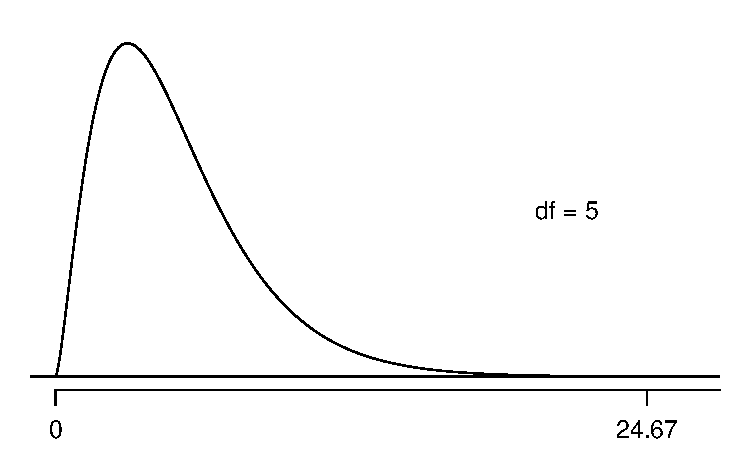
\includegraphics[width=0.67\textwidth]{6-3_chisq_gof/above24Point67WithDF5.pdf}
\end{center}
}
{
p-valor = $P(\chi^2_{df = 5} > 24.67)$\\ é menos do que 0.001
}
\end{frame}
%%%%%%%%%%%%%%%%%%%%%%%%%%%%%%%%%%%

\begin{frame}
\frametitle{Encontrar o p-valor de um teste do qui-quadrado}

\begin{center}
{\scalefont{0.7}
\begin{tabular}{r | rrrr | rrrr r}
  \hline
Cauda superior & 0.3 & 0.2 & 0.1 & 0.05 & 0.02 & 0.01 & 0.005 & 0.001 & \orange{$\rightarrow$}  \\ 
  \hline
df \hfill 1 &  1.07 &  1.64 &  2.71 &  3.84 &  5.41 &  6.63 &  7.88 &  10.83 \\ 
  2 &  2.41 &  3.22 &  4.61 &  5.99 &  7.82 &  9.21 &  10.60 &  13.82 \\ 
  3 &  3.66 &  4.64 &  6.25 &  7.81 &  9.84 &  11.34 &  12.84 &  16.27 \\ 
  4 &  4.88 &  5.99 &  7.78 &  9.49 &  11.67 &  13.28 &  14.86 &  18.47 \\ 
  \rowcolor[gray]{.6}
  5 &  6.06 &  7.29 &  9.24 &  11.07 &  13.39 &  15.09 &  16.75 &  20.52 &\orange{$\rightarrow$} \\ 
  \hline
\end{tabular}
}
\end{center}

\end{frame}

%%%%%%%%%%%%%%%%%%%%%%%%%%%%%%%%%%%

\begin{frame}
\frametitle{Conclusão do teste de hipóteses}
\justifying
\pq{Calculamos um p-valor menor que 0.001. Ao nível de significância de 5\%, qual é a conclusão do teste de hipótese?}

\begin{enumerate}[(a)]
\justifying
\item Rejeitar $H_0$, os dados fornecem evidências convincentes de que os dados são honestos.
\justifying
\solnMult{Rejeitar $H_0$, os dados fornecem evidências convincentes de que os dados são tendenciosos.}
\justifying
\item Não rejeitar $H_0$, os dados fornecem evidências convincentes de que os dados são honestos.
\justifying
\item Não rejeitar $H_0$, os dados fornecem evidências convincentes de que os dados são tendenciosos.
\end{enumerate}

\end{frame}

%%%%%%%%%%%%%%%%%%%%%%%%%%%%%%%%%%%

\begin{frame}
\frametitle{Acontece que...}

\begin{itemize}
\justifying
\item O eixo 1-6 é consistentemente mais curto que os outros dois (2-5 e 3-4), suportando assim a hipótese de que as faces com 1 e 6 são maiores que as outras faces.
\justifying
\item A alegação de Pearson de que 5s e 6s aparecem com mais frequência devido aos pips esculpidos não é suportada por esses dados.
\justifying
\item Os dados usados nos cassinos têm faces niveladas, onde os pontos são preenchidos com um plástico da mesma densidade do material circundante e são precisamente balanceados.

\end{itemize}

\begin{center}
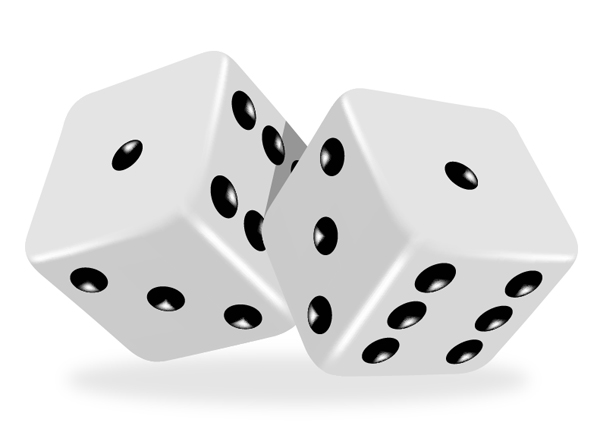
\includegraphics[width=0.3\textwidth]{6-3_chisq_gof/regular.jpeg}
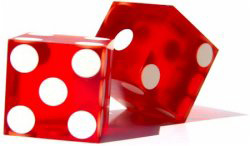
\includegraphics[width=0.3\textwidth]{6-3_chisq_gof/casino.jpeg}
\end{center}


\end{frame}

%%%%%%%%%%%%%%%%%%%%%%%%%%%%%%%%%%%

\begin{frame}
\frametitle{Recapitulando: p-valor do teste qui-quadrado}

\begin{itemize}
\justifying
\item O p-valor do teste qui-quadrado é definido como a área de cauda \hl{acima} da estatística de teste calculada.
\justifying
\item Isso ocorre porque a estatística de teste é sempre positiva e uma estatística de teste mais alta significa um desvio maior da hipótese nula.

\end{itemize}

\begin{center}
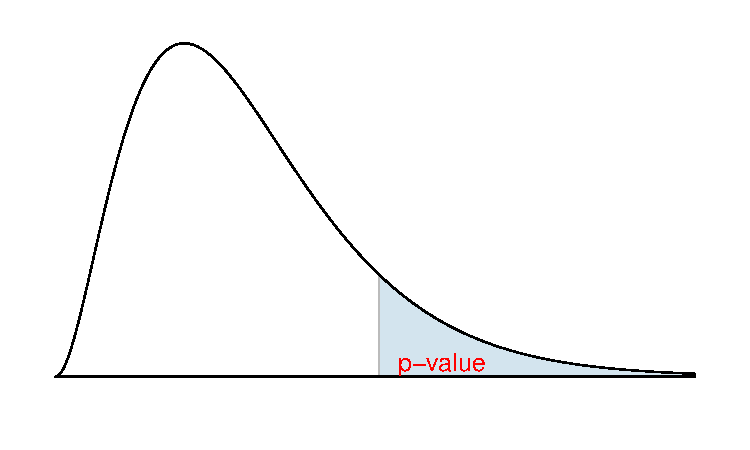
\includegraphics[width=0.7\textwidth]{6-3_chisq_gof/genericChiSquare.pdf}
\end{center}

\end{frame}

%%%%%%%%%%%%%%%%%%%%%%%%%%%%%%%%%%%

\begin{frame}
\frametitle{Condições para o teste do qui-quadrado}

\begin{enumerate}
\justifying
\item \hlGr{Independência:} Cada caso que contribui com uma contagem para a tabela deve ser independente de todos os outros casos na tabela.

\pause
\justifying
\item \hlGr{Tamanho da amostra:} Cada cenário específico (ou seja, cada célula) deve ter pelo menos 5 casos \orange{esperados}.

\pause
\justifying
\item \hlGr{df $>$ 1:} Graus de liberdade devem ser maiores que 1.

\end{enumerate}

\pause
\justifying
Deixar de verificar as condições pode afetar as taxas de erro do teste.

\end{frame}

%%%%%%%%%%%%%%%%%%%%%%%%%%%%%%%%%%%

\subsection{Eleição de 2009 Irã}

%%%%%%%%%%%%%%%%%%%%%%%%%%%%%%%%%%%

\begin{frame}
\frametitle{Eleição de 2009 no Irã}
\justifying
\dq{Falou-se muito sobre fraude eleitoral nas eleições de 2009 no Irã. Vamos comparar os dados de uma pesquisa realizada antes da eleição (dados observados) com os votos informados na eleição para ver se os dois seguem a mesma distribuição.}

\begin{center}
\begin{tabular}{l | r r}
					& \footnotesize{\# observado de} & \footnotesize{\% relatada de} \\
\footnotesize{Candidato}	& \footnotesize{votos na pesquisa} & \footnotesize{votos na eleição} \\
\hline
(1) Ahmedinajad	& 338	& 63.29\% \\
(2) Mousavi		& 136	& 34.10\% \\
(3) Candidatos menores	& 30	& 2.61\% \\
\hline
Total			& 504	& 100\% \\
\pause
			& \hl{$\downarrow$}	& \hl{$\downarrow$}	\\
			& \hl{observado}	& \hl{esperado} \\
			& 			& \hl{distribuição} 	
\end{tabular}
\end{center}

\end{frame}

%%%%%%%%%%%%%%%%%%%%%%%%%%%%%%%%%%%

\begin{frame}
\frametitle{Hipóteses}
\justifying
\dq{Quais são as hipóteses para testar se as distribuições de votos informados e observados são diferentes?}

\soln{
\only<2>{
\begin{itemize}
\justifying
\item[$H_0$:] As contagens observadas da pesquisa seguem a mesma distribuição dos votos relatados.
\justifying
\item[$H_A$:] As contagens observadas da pesquisa não seguem a mesma distribuição que os votos relatados.
\end{itemize}
}}

\end{frame}

%%%%%%%%%%%%%%%%%%%%%%%%%%%%%%%%%%%

\begin{frame}
\frametitle{Cálculo da estatística de teste}


\begin{center}
\scalefont{0.7}
\begin{tabular}{l | r r r}
					& \# observado de & \% relatada de	& \# esperado de \\
Candidato	& votos na pesquisa & votos na eleição		&  votos na pesquisa \\
\hline
(1) Ahmedinajad	& 338	& 63.29\% 	& 504 $\times$ 0.6329 = 319 \\
(2) Mousavi		& 136	& 34.10\%		& 504 $\times$ 0.3410 = 172 \\
(3) Candidatos menores	& 30	& 2.61\% 		& 504 $\times$ 0.0261 = 13\\
\hline
Total			& 504	& 100\%		& 504
\end{tabular}
\end{center}


\pause

\begin{eqnarray*}
\frac{(O_1 - E_1)^2}{E_1} = \frac{(338 - 319)^2}{319} &=& 1.13 \\
\pause
\frac{(O_2 - E_2)^2}{E_2} = \frac{(136 - 172)^2}{172} &=& 7.53 \\
\pause
\frac{(O_2 - E_2)^2}{E_2} = \frac{(30 - 13)^2}{13} &=& 22.23 \\
\pause
 \chi^2_{\mathhl{df = 3 - 1 = 2}} &=& 30.89
\end{eqnarray*}


\end{frame}

%%%%%%%%%%%%%%%%%%%%%%%%%%%%%%%%%%%

\begin{frame}
\frametitle{Conclusão}
\justifying
\pq{Com base nesses cálculos, qual é a conclusão do teste de hipóteses?}

\begin{enumerate}[(a)]
\justifying
\solnMult{o p-valor é baixo, $H_0$ é rejeitada. As contagens observadas na pesquisa \underline {não} seguem a mesma distribuição que os votos relatados.}
\justifying
\item o p-valor é alto, $H_0$ não é rejeitada. As contagens observadas na pesquisa seguem a mesma distribuição dos votos relatados.
\justifying
\item o p-valor é baixo, $H_0$ é rejeitada. As contagens observadas na pesquisa seguem a mesma distribuição que os votos relatados.
\justifying
\item o p-valor é baixo, $H_0$ não é rejeitada. As contagens observadas na pesquisa \underline {não} seguem a mesma distribuição que os votos relatados.
\end{enumerate}

\end{frame}
%%%%%%%%%%%%%%%%%%%%%%%%%%%%%%%%%%%%

\section{6.4. Teste de independência de qui-quadrado}

%%%%%%%%%%%%%%%%%%%%%%%%%%%%%%%%%%%

\subsection{Crianças populares}

%%%%%%%%%%%%%%%%%%%%%%%%%%%%%%%%%%%

\begin{frame}
\frametitle{Crianças populares}
\justifying
\dq{No conjunto de dados \texttt{popular}, os alunos das 4ª a 6ª séries foram questionados se boas notas, ser atlético ou ser popular era mais importante para eles. Uma tabela de duas vias que separa os alunos por série e por escolha do fator mais importante é mostrada abaixo. Esses dados fornecem evidências para sugerir que as preferências variam de acordo com o série?
}

\twocol{0.5}{0.5}
{
\begin{center}
\begin{tabular}{rrrr}
  \hline
 & Notas & Popular & Esportes \\ 
  \hline
$4^{a}$ &  63 &  31 &  25 \\ 
$5^{a}$ &  88 &  55 &  33 \\ 
$6^{a}$ &  96 &  55 &  32 \\ 
   \hline
\end{tabular}
\end{center}
}
{
\begin{center}
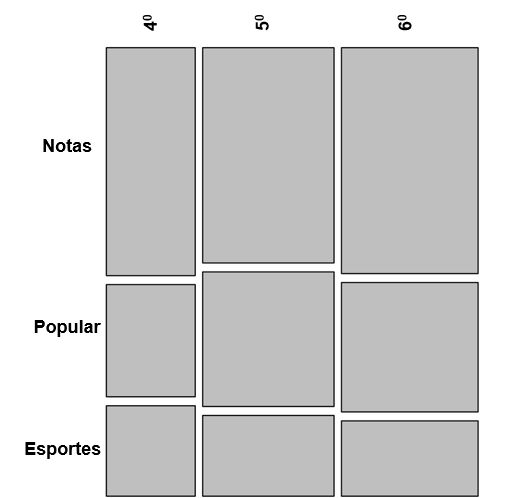
\includegraphics[width=0.8\textwidth]{6-4_chisq_indep/popular_mosaic.png}
\end{center}
}


\end{frame}

%%%%%%%%%%%%%%%%%%%%%%%%%%%%%%%%%%%

\begin{frame}
\frametitle{Teste de independência do qui-quadrado}

\begin{itemize}
\justifying
\item As hipóteses são:
\begin{itemize}
\justifying
\item[$H_0$:] A série e as preferências são independentes. As preferências não variam de acordo com a série.
\justifying
\item[$H_A$:] A série e as preferências são dependentes. As preferências variam de acordo com a série.
\end{itemize}

\pause
\justifying
\item A estatística de teste é calculada como
\[ \chi^2_{df} = \sum_{i = 1}^{k} \frac{(O - E)^2}{E} \quad \text{ onde } \quad df = (R - 1) \times (C - 1), \]
onde $k$ é o número de células, $ R $ é o número de linhas e $ C $ é o número de colunas.\\

\pause
\justifying
\item O p-valor é a área sob a curva $\chi^2_{df}$ acima da estatística de teste calculada.


\justifying
\tiny{\Note{Calculamos $df$ de forma diferente para tabelas de uma via e duas vias.}}



\end{itemize}


\end{frame}

%%%%%%%%%%%%%%%%%%%%%%%%%%%%%%%%%%%

\subsection{Contagens esperadas em tabelas de duas vias}

%%%%%%%%%%%%%%%%%%%%%%%%%%%%%%%%%%%

\begin{frame}
\frametitle{Contagens esperadas em tabelas de duas vias}
\justifying
\formula{Contagens esperadas em tabelas de duas vias}
{
\[ \text{Contagem esperada} = \frac{(\text{total da linha}) \times (\text{total da coluna})}{\text{total da tabela}} \]
}

\pause

{\small
\begin{center}
\begin{tabular}{rrrr|r}
  \hline
 & Notas & Popular & Esportes	& Total \\ 
  \hline
$4^{a}$ &  \orange{63} &  \green{31} &  25 	&119 \\ 
$5^{a}$ &  88 &  55 &  33	& 176 \\ 
$6^{a}$&  96 &  55 &  32	& 183 \\ 
   \hline
Total	& 247	& 141	& 90	& 478 \\
\end{tabular}
\end{center}
}

\pause

\[ \orange{$E_{linha~1, coluna~1} = \frac{119 \times 247}{478} = 61$} \qquad \pause
 \green{$E_{linha~1, coluna~2} = \frac{119 \times 141}{478} = 35$} \]

\end{frame}

%%%%%%%%%%%%%%%%%%%%%%%%%%%%%%%%%%%

\begin{frame}
\frametitle{Contagens esperadas em tabelas bidirecionais}
\justifying
\pq{Qual é a contagem esperada para a célula realçada?}

{\small
\begin{center}
\begin{tabular}{rrrr|r}
  \hline
 & Notas & Popular & Esportes	& Total \\ 
  \hline
$4^{a}$ &  63 &  31 &  25 	&119 \\ 
$5^{a}$ &  88 &  55 &  33   &176\\ 
$6^{a}$ &  96 &  55 &  32	& 183 \\ 
   \hline
Total	& 247	& 141	& 90	& 478 \\
\end{tabular}
\end{center}
}

\twocol{0.2}{0.8}
{
\begin{enumerate}[(a)]
\solnMult{$\frac{176 \times 141}{478}$}
\item $\frac{119 \times 141}{478}$
\item $\frac{176 \times 247}{478}$
\item $\frac{176 \times 478}{478}$
\end{enumerate}
}
{
\soln{\only<2>{\justifying
\orange{$\rightarrow$ 52\\
{\small mais do que o \# esperado de alunos do 5º ano \\
tem preferência por ser popular}}
\vspace{0.75cm}
}
}
}

\end{frame}

%%%%%%%%%%%%%%%%%%%%%%%%%%%%%%%%%%%

\begin{frame}
\frametitle{Calculando a estatística de teste em tabelas bidirecionais}
\justifying
As contagens esperadas são mostradas em \ex {azul} ao lado das contagens observadas.
\begin{center}
\begin{tabular}{rrrr|r}
  \hline
 & Notas & Popular & Esportes	& Total \\ 
  \hline
$4^{a}$ 	&  63 \ex{61} &  31 \ex{35} &  25 \ex{23}	&119 \\ 
$5^{a}$ 	&  88 \ex{91} &  55 \ex{52} &  33 \ex{33}	& 176 \\ 
$6^{a}$	&  96 \ex{95} &  55 \ex{54} &  32 \ex{34}	& 183 \\ 
   \hline
Total	& 247	& 141	& 90	& 478 \\
\end{tabular}
\end{center}

\vspace{0.5cm}

\pause

\begin{eqnarray*} 
\chi^2 &=& \sum \frac{(63 - 61)^2}{61} + \frac{(31 - 35)^2}{35} + \cdots + \frac{(32 - 34)^2}{34} = 1.3121 \\
\pause
df &=& (R - 1) \times (C - 1) = (3 - 1) \times (3 - 1) = 2 \times 2 = 4 
\end{eqnarray*}

\end{frame}

%%%%%%%%%%%%%%%%%%%%%%%%%%%%%%%%%%%

\subsection{Resultados}

%%%%%%%%%%%%%%%%%%%%%%%%%%%%%%%%%%%

\begin{frame}
\frametitle{Calculando o p-valor}
\justifying
\pq{Qual dos seguintes é o p-valor correto para este teste de hipóteses?
\[ \chi^2 = 1.3121 \qquad df = 4 \]
}

\twocol{0.6}{0.4}{
\begin{center}
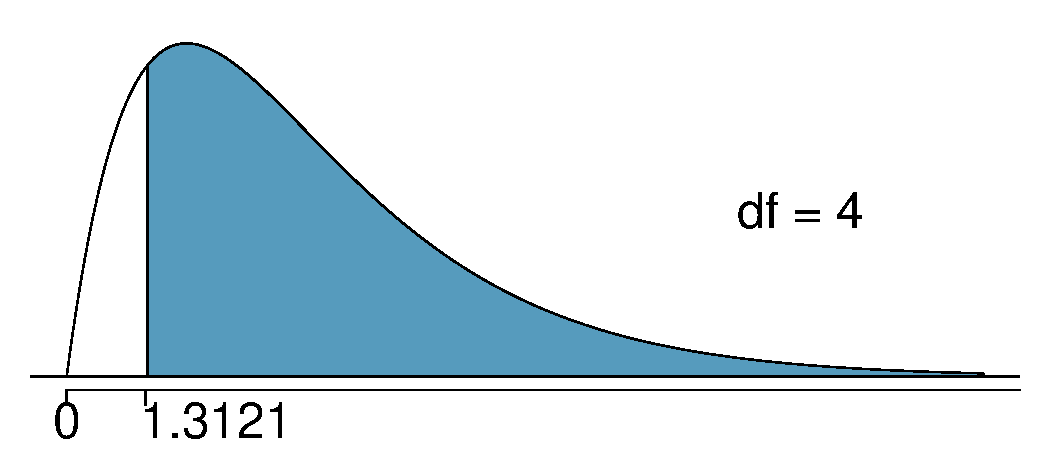
\includegraphics[width=0.67\textwidth]{6-4_chisq_indep/popular.pdf}
\end{center}
}
{
{\small
\begin{enumerate}[(a)]
\setlength{\itemsep}{0in}
\solnMult{ maior que 0.3}
\item entre 0.3 e 0.2
\item entre 0.2 e 0.1
\item entre 0.1 e 0.05
\item menor que 0.001
\end{enumerate}
}
}
\end{frame}
%%%%%%%%%%%%%%%%%%%%%%%%%%%%%%%%%%%

\begin{frame}
\frametitle{Calculando o p-valor}

\begin{center}
{\scriptsize
\begin{tabular}{r | rrrr | rrrr |}
  \hline
Cauda superior & 0.3 & 0.2 & 0.1 & 0.05 & 0.02 & 0.01 & 0.005 & 0.001 \\ 
  \hline
df \hfill 1 &  1.07 &  1.64 &  2.71 &  3.84 &  5.41 &  6.63 &  7.88 &  10.83 \\ 
  2 &  2.41 &  3.22 &  4.61 &  5.99 &  7.82 &  9.21 &  10.60 &  13.82 \\ 
  3 &  3.66 &  4.64 &  6.25 &  7.81 &  9.84 &  11.34 &  12.84 &  16.27 \\ 
  4 &  4.88 &  5.99 &  7.78 &  9.49 &  11.67 &  13.28 &  14.86 &  18.47 \\ 
  5 &  6.06 &  7.29 &  9.24 &  11.07 &  13.39 &  15.09 &  16.75 &  20.52 \\ 
\end{tabular}
}
\end{center}

\end{frame}

%%%%%%%%%%%%%%%%%%%%%%%%%%%%%%%%%%%

\begin{frame}
\frametitle{Conclusão}
\justifying
\dq{Esses dados fornecem evidências para sugerir que as preferências variam de acordo com a série?}

\begin{itemize}
\justifying
\item[$H_0$:] A série e as preferências são independentes. As preferências não variam de acordo com a séries.
\justifying
\item[$H_A$:] A série e as preferências são dependentes. As preferências variam de acordo com a série. \\

\end{itemize}

$\:$ \\
\justifying
\soln{\only<2>{Como o p-valor é alto, não rejeitamos $H_0$. Os dados não fornecem evidências convincentes de que a série e as preferências são dependentes. Não parece que as preferências variam por série.
}
}

\end{frame}
%%%%%%%%%%%%%%%%%%%%%%%%%%%%%%%%%%%%

\section{6.5. Inferência para uma proporção com uma amostra pequena}

%%%%%%%%%%%%%%%%%%%%%%%%%%%%%%%%%%%%

\subsection{Paul, o polvo}

%%%%%%%%%%%%%%%%%%%%%%%%%%%%%%%%%%%%

\begin{frame}
\frametitle{Preditores famosos}

\twocol{0.5}{0.5}{
Antes desse cara...
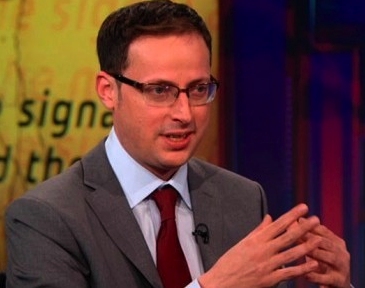
\includegraphics[width=\textwidth]{6-5_small_single_prop/nate.png}
}
{
\pause
Tinha esse cara...
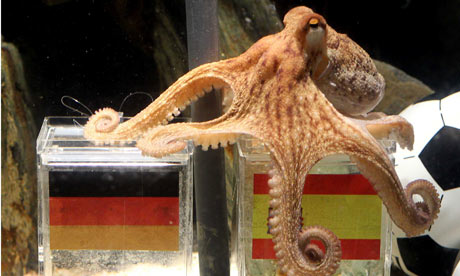
\includegraphics[width=\textwidth]{6-5_small_single_prop/paul.png}
}

\end{frame}

%%%%%%%%%%%%%%%%%%%%%%%%%%%%%%%%%%

\begin{frame}
\frametitle{Paul, o polvo - psíquico?}

\begin{itemize}
\justifying
\item Paul, o polvo, previu 8 jogos da Copa do Mundo corretamente.

\pause
\justifying
\item Isso fornece evidências convincentes de que Paul realmente tem poderes psíquicos?

\pause
\justifying
\item Quão incomum seria se ele estivesse apenas adivinhando aleatoriamente (com 50\% de chance de
adivinhar corretamente)?

\pause
\justifying
\item Hipóteses:
\begin{itemize}
\item[$H_0:$] $p = 0.5$
\item[$H_A:$] $p > 0.5$
\end{itemize}

\end{itemize}

\end{frame}

%%%%%%%%%%%%%%%%%%%%%%%%%%%%%%%%%%

\begin{frame}
\frametitle{Condições}

\begin{enumerate}
\justifying
\item \hl{Independência:} Podemos supor que cada palpite é independente de outro.

\pause
\justifying
\item \hl{Tamanho da amostra:} O número de sucessos esperados é \orange{menor que 10}.
\[ 8 \times 0.5 = 4 \]

\end{enumerate}

\pause

\vspace{1cm}
\justifying
\dq{Então, o que fazemos?}

\pause
\justifying
Como o tamanho da amostra não é grande o suficiente para usar métodos baseados em TCL, usamos um método de simulação.

\end{frame}

%%%%%%%%%%%%%%%%%%%%%%%%%%%%%%%%%%

\begin{frame}
\frametitle{Prática}
\justifying
\pq{Qual dos seguintes métodos é a melhor maneira de calcular o p-valor do teste de hipótese para testar se as previsões de Paul, o polvo, são excepcionalmente mais altas do que adivinhações aleatórias?}

\scalefont{0.8}
\begin{enumerate}[(a)]
\justifying
\item Jogue uma moeda 8 vezes, registre a proporção de vezes em que todos os 8 lançamentos foram cara. Repita isso muitas vezes e calcule a proporção de simulações em que todos os 8 lançamentos foram cara.
\justifying
\item Jogue um dado 8 vezes, registre a proporção de vezes em que todos os 8 lançamentos foram 6s. Repita isso várias vezes e calcule a proporção de simulações em que todos os 8 lançamentos foram 6s.
\justifying
\item Jogue uma moeda 10.000 vezes, registre a proporção de cara. Repita isso várias vezes e calcule a proporção de simulações em que mais de 50\% dos lançamentos são cara.
\justifying
\item Jogue uma moeda 10.000 vezes, calcule a proporção de cara.
\end{enumerate}

\end{frame}

%%%%%%%%%%%%%%%%%%%%%%%%%%%%%%%%%%%

\begin{frame}
\frametitle{Simular}
\justifying
\pq{Jogue uma moeda 8 vezes. Você conseguiu todas as caras?}

\begin{enumerate}[(a)]
\item Sim
\item Não
\end{enumerate}

\end{frame}

%%%%%%%%%%%%%%%%%%%%%%%%%%%%%%%%%%

\begin{frame}[fragile]
\frametitle{Simular}
\justifying
{\tiny
\begin{Verbatim}[frame=single, formatcom=\color{blue}]
fonte ("http://www.openintro.org/stat/slides/inference.R")
paul = fator(c(rep("sim", 8), rep("não", 0)), nível = c("sim","não"))
inferência(paul, est = "proporção", tipo = "ht", método = "simulação",
          sucesso = "sim", nulo = 0.5, alternativo = "maior", semente = 290)
\end{Verbatim}
}

\pause
\justifying
{\tiny
\begin{Verbatim}[frame=single, formatcom=\color{gray}]
Proporção única -- sucesso: sim
Estatísticas resumidas: p_hat = 1 ;  n = 8 
H0: p = 0.5 
HA: p > 0.5 
valor-p =  0.0037
\end{Verbatim}
}

\centering
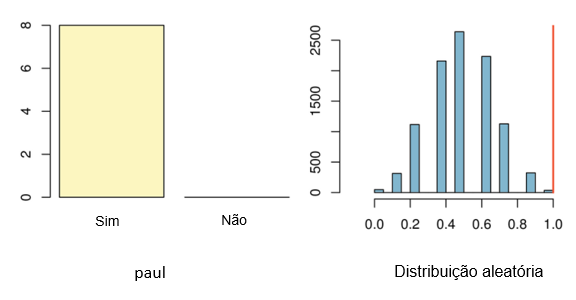
\includegraphics[width=0.8\textwidth,height=0.4\textheight]{6-5_small_single_prop/paul_HT.png}

\end{frame}

%%%%%%%%%%%%%%%%%%%%%%%%%%%%%%%%%%%

\begin{frame}
\frametitle{Conclusões}
\justifying
\pq{Qual das seguintes opções é \underline {falsa}??}

\begin{enumerate}[(a)]
\justifying
\item Se, de fato, Paul estivesse adivinhando aleatoriamente, a probabilidade de ele obter o resultado de todos os 8 jogos corretos é 0,0037.
\justifying
\item Rejeitar $H_0$, os dados fornecem evidências convincentes de que Paul fez mais do que adivinhar aleatoriamente.
\justifying
\item Podemos ter cometido um erro do Tipo I.

\solnMult{A probabilidade de que Paul seja psíquico é 0,0037.}

\end{enumerate}

\end{frame}

%%%%%%%%%%%%%%%%%%%%%%%%%%%%%%%%%%%%

\subsection{Dorso da mão}

%%%%%%%%%%%%%%%%%%%%%%%%%%%%%%%%%%%

\begin{frame}
\frametitle{Dorso da mão}
\justifying
\dq{Há um ditado que diz "conheça algo como a palma da sua mão". Descreva um experimento para testar se as pessoas conhecem \textit{o dorso} de suas mãos.}

\pause

\begin{center}
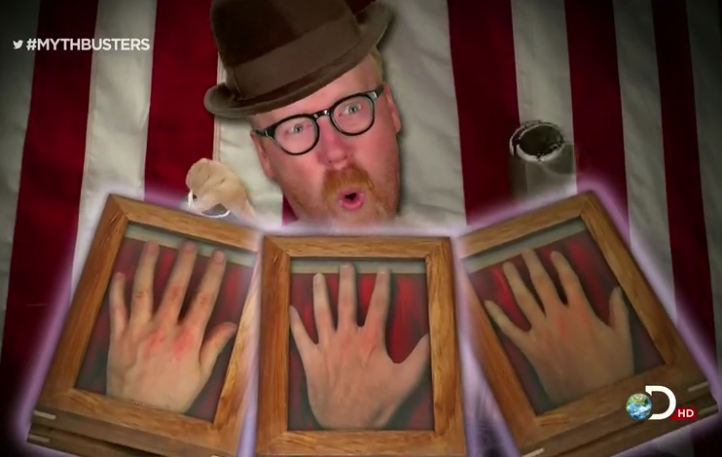
\includegraphics[width=0.6\textwidth]{6-5_small_single_prop/mythbusters.png}
\end{center}
\justifying
No episódio de MythBusters, 11 de 12 pessoas adivinham as costas de suas mãos corretamente.

\end{frame}

%%%%%%%%%%%%%%%%%%%%%%%%%%%%%%%%%%%%

\begin{frame}
\frametitle{Hipóteses}
\justifying
\dq{Quais são as hipóteses para avaliar se as pessoas são capazes de reconhecer o dorso da mão a uma taxa melhor que uma adivinhação aleatória. Lembre-se, no experimento do MythBusters, havia 10 fotos para escolher, e apenas 1 estava correta.}

\begin{itemize}
\item[$H_0:$] $p = 0.10$ (adivinhação aleatória)
\item[$H_A:$] $p > 0.10$ (mais do que adivinhar aleatoriamente)
\end{itemize}

\end{frame}

%%%%%%%%%%%%%%%%%%%%%%%%%%%%%%%%%%%

\begin{frame}
\frametitle{Condições}

\begin{enumerate}
\justifying
\item \hl{Independência:} Podemos supor que cada pessoa que adivinhando é independente de outra.
\justifying
\item \hl{Tamanho da amostra:} O número de sucessos esperados é \orange{menor que 10}.
\[ 12 \times 0.1 = 1.2 \]

\end{enumerate}
\justifying
\dq{Então, o que fazemos?}
\justifying
Como o tamanho da amostra não é grande o suficiente para usar métodos baseados em TCL, usamos um método de simulação.

\end{frame}

%%%%%%%%%%%%%%%%%%%%%%%%%%%%%%%%%%%

\subsection{Aleatorização HT para uma proporção}

%%%%%%%%%%%%%%%%%%%%%%%%%%%%%%%%%%%%

\begin{frame}
\frametitle{Esquema de simulação}
\justifying
\dq{Descreva como você testaria se os resultados desse experimento determinam se as pessoas são capazes de reconhecer o dorso da mão a uma taxa melhor do que uma adivinhação aleatória.}
\vspace{-0.5cm}
\[ H_0: p = 0.10 \qquad H_A: p > 0.10 \qquad \hat{p} = 11 / 12 = 0.9167 \]

\scalefont{0.7}
\begin{enumerate}
\justifying
\item Use um dado justo de 10 lados para representar o espaço de amostragem, e chame 1 de sucesso (adivinhando corretamente), e todas os outros resultados de falhas (adivinhando incorretamente).

\justifying
\item Jogue o dado 12 vezes (representando 12 pessoas no experimento), conte o número de 1s e calcule a proporção de palpites corretos em uma simulação com 12 lançamentos.
\justifying
\item Repita o passo (2) muitas vezes, registrando a proporção de sucessos em uma série de 12 lançamentos do dado.
\justifying
\item Crie um gráfico de pontos das proporções simuladas a partir do passo (3) e conte o número de simulações em que a proporção foi pelo menos tão alta quanto 0.9167 (a proporção observada).

\end{enumerate}

\end{frame}

%%%%%%%%%%%%%%%%%%%%%%%%%%%%%%%%%%%

\begin{frame}
\frametitle{Resultados simulados}

\begin{itemize}
\justifying
\item No próximo slide você pode ver os resultados de um teste de hipótese (usando apenas 100 simulações para manter as coisas simples).
\justifying
\item Cada ponto representa uma proporção de sucesso da simulação. Houve 25-30 simulações em que a taxa de sucesso ($\hat{p}$) foi de 10\%, 40-45 simulações em que a taxa de sucesso foi ligeiramente inferior a 10\%, cerca de 20 simulações em que a taxa de sucesso foi ligeiramente menor que 20\% e 1 simulação em que a taxa de sucesso foi superior a 30\%.
\justifying
\item Não há simulações em que a taxa de sucesso seja tão alta quanto a taxa de sucesso observada de 91.67\%.

\end{itemize}
\end{frame}

%%%%%%%%%%%%%%%%%%%%%%%%%%%%%%%%%%%

\begin{frame}
\frametitle{Resultados simulados}

\begin{itemize}
\justifying
\item Portanto, concluímos que o resultado observado é quase impossível de acontecer por acaso (p-valor = 0).
\justifying
\item E, portanto, esses dados sugerem que as pessoas são capazes de reconhecer as costas de suas mãos a uma taxa melhor do que adivinhar aleatoriamente.

\end{itemize}

\end{frame}

%%%%%%%%%%%%%%%%%%%%%%%%%%%%%%%%%%%%

\begin{frame}[fragile]
\frametitle{Resultados simulados}
\justifying
{\tiny
\begin{Verbatim}[frame=single, formatcom=\color{blue}]
costas = as.factor(c(rep("correto", 11), rep("errado", 1))) 
inferência(costas, est = "proporção", tipo = "ht", método = "simulação",
	sucesso = "correto", nulo = 0.1, alternativo = "maior", semente = 654, nsim = 100)
\end{Verbatim}
}

\pause
\justifying
{\tiny
\begin{Verbatim}[frame=single, formatcom=\color{gray}]
Proporção única - sucesso: correto 
Estatísticas resumidas: p_hat = 0.9167 ;  n = 12 
H0: p = 0.1 
HA: p > 0.1 
p-value =  0 
\end{Verbatim}
}

\centering
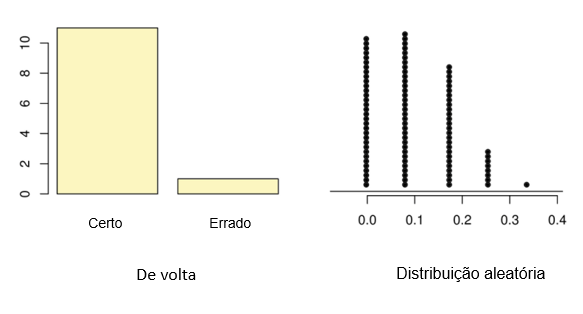
\includegraphics[width=0.8\textwidth,height=0.4\textheight]{6-5_small_single_prop/back_HT.png}

\end{frame}

%%%%%%%%%%%%%%%%%%%%%%%%%%%%%%%%%%%

%%%%%%%%%%%%%%%%%%%%%%%%%%%%%%%%%%%%
\justifying
\section{6.6. Inferência para diferença entre duas proporções com uma amostra pequena}

%%%%%%%%%%%%%%%%%%%%%%%%%%%%%%%%%%%%

\begin{frame}
\frametitle{Comparando as costas da mão à palma da mão}
\justifying
MythBusters também pediu a essas pessoas para adivinharem as palmas das mãos. Desta vez, 7 das 12 pessoas acertaram. Os dados estão resumidos abaixo.

\begin{center}
\begin{tabular}{ l | c | c | c }
          & Dorso		& Palma		& Total \\
\hline
Correto		& 11			& 7				& 18 \\
Errado		  & 1				& 5				& 6 \\
\hline
Total			& 12			& 12			& 24 \\
\end{tabular}
\end{center}

\end{frame}

%%%%%%%%%%%%%%%%%%%%%%%%%%%%%%%%%%%%

\begin{frame}
\frametitle{Proporção de palpites corretos}

{\small
\begin{center}
\begin{tabular}{ l | c | c | c }
          & Dorso  	& Palma		& Total \\
\hline
Correto		& 11			& 7				& 18 \\
Errado		  & 1				& 5				& 6 \\
\hline
Total			& 12			& 12			& 24 \\
\end{tabular}
\end{center}

}

\begin{itemize}
\justifying
\item Proporção de acertos no grupo do dorso: $\frac{11}{12} = 0.916$
\justifying
\item Proporção de correto no grupo da palme: $\frac{7}{12} = 0.583$
\justifying
\item Diferença: 33.3\% mais acertos do grupo que avaliou o dorso das mãos.

\end{itemize}
\justifying
\dq{Com base nas proporções calculadas, você acha que a chance de adivinhar corretamente o dorso da mão é diferente da palma da mão?}

\end{frame}

%%%%%%%%%%%%%%%%%%%%%%%%%%%%%%%%%%%%

\begin{frame}
\frametitle{Hipóteses}
\justifying
\dq{Quais são as hipóteses para comparar se a proporção de pessoas que conseguem adivinhar corretamente o dorso de suas mãos é diferente da proporção de pessoas que conseguem adivinhar corretamente a palma de suas mãos?}

\begin{itemize}
\item[$H_0$:] $p_{dorso} = p_{palma}$
\item[$H_0$:] $p_{dorso} \ne p_{palma}$
\end{itemize}

\end{frame}

%%%%%%%%%%%%%%%%%%%%%%%%%%%%%%%%%%%%

\begin{frame}
\frametitle{Condições?}

\begin{itemize}
\justifying
\item Independência - dentro de grupos, entre grupos?
\begin{itemize}
\justifying
\item Dentro de cada grupo podemos supor que o palpite de um sujeito é independente do outro.
\justifying
\item Entre os grupos, a independência não é satisfeita - temos as mesmas pessoas adivinhando. No entanto, vamos supor que são suposições independentes para continuar com a análise.
\end{itemize}
\justifying
\item Tamanho da amostra?
\begin{itemize}
\justifying
\item $\hat{p}_{amostra} = \frac{11 + 7}{12 + 12} = \frac{18}{24} = 0.75$.
\justifying
\item Sucessos esperados no grupo do dorso: $ 12 \times 0.75 = 9 $, falhas = 3.
\justifying
\item Sucessos esperados no grupo da palma: $ 12 \times 0.75 = 9 $, falhas = 3.
\justifying
\item Como a condição Sucessos/Fracassos falha, precisamos usar a simulação para comparar as proporções.
\end{itemize}

\end{itemize}

\end{frame}

%%%%%%%%%%%%%%%%%%%%%%%%%%%%%%%%%%%%

\subsection{Aleatorização HT para comparar duas proporções}

%%%%%%%%%%%%%%%%%%%%%%%%%%%%%%%%%%%%

\begin{frame}
\frametitle{Esquema de simulação}

\begin{enumerate}
\justifying
\item Use 24 fichas de índice, onde cada cartão representa um assunto.
\justifying
\item Marque 18 das cartas como "corretas" e as 6 restantes como "erradas".
\justifying
\item Embaralhe as cartas e divida em dois grupos de tamanho 12, para as costas e a palma da mão.
\justifying
\item Calcule a diferença entre as proporções de "correto para o dorso" e nos decks de palma, e registre este número.
\justifying
\item Repita as etapas (3) e (4) várias vezes para criar uma distribuição aleatória das diferenças nas proporções simuladas.

\end{enumerate}

\end{frame}

%%%%%%%%%%%%%%%%%%%%%%%%%%%%%%%%%%%%

\begin{frame}
\frametitle{Interpretando os resultados da simulação}
\justifying
Simulando o experimento sob o pressuposto de independência, ou seja, deixando as coisas ao acaso. \\

\vspace{0.5cm}
\justifying
Se os resultados das simulações baseadas no modelo nulo se parecem com os dados, então podemos determinar que a diferença entre as proporções das estimativas corretas nos dois grupos foi simplesmente \hl{devido ao acaso}. \\

\vspace{0.5cm}
\justifying
Se os resultados das simulações baseadas no modelo nulo não se parecem com os dados, então podemos determinar que a diferença entre as proporções dos palpites corretos nos dois grupos não foi devida ao acaso, mas \hl{sim porque as pessoas realmente conhecem o dorso de suas mãos melhor do que a palma}.

\end{frame}

%%%%%%%%%%%%%%%%%%%%%%%%%%%%%%%%%%%%

\begin{frame}
\frametitle{Resultados simulados}

\begin{itemize}
\justifying
\item No próximo slide você pode ver o resultado de um teste de hipótese (usando apenas 100 simulações para manter os resultados simples).
\justifying
\item Cada ponto representa uma diferença na proporção simulada de sucessos. Podemos ver que a distribuição está centrada em 0 (o valor nulo).
\justifying
\item Também podemos ver que 9 das 100 simulações produziram diferenças simuladas pelo menos tão grandes quanto a diferença observada (p-valor = 0.09).

\end{itemize}

\end{frame}

%%%%%%%%%%%%%%%%%%%%%%%%%%%%%%%%%%%%

\begin{frame}[fragile]
\frametitle{Simulação}

{\tiny
\begin{Verbatim}[frame=single, formatcom=\color{blue}]
mão = as.factor (c (rep ("correto", 7), rep ("errado", 5), c (rep ("correto", 11), rep ("errado", 1))))
gr = c(rep("palma",12),rep("dorso",12))
inferência (mão, gr, est = "proporção", tipo = "ht", null = 0, alternativa = "twosided",
	order = c ("voltar", "palma"), sucesso = "correto", método = "simulação", semente = 879,
	nsim = 100)
\end{Verbatim}
}

\pause

{\tiny
\begin{Verbatim}[frame=single, formatcom=\color{gray}]
Variável de resposta: categórica, Variável explicativa: categórica
Diferença entre duas proporções - sucesso: correto
Estatísticas resumidas:
         x
y         soma  palma  dorso
  correto   11    7  18
  errado      1    5   6
  soma       12   12  24
Diferença observada entre proporções (palma da mão) = 0.3333
H0: dorso - p_palma = 0 
HA: p_dorso - p_palma != 0 
valor-p =  0.18 
\end{Verbatim}
}

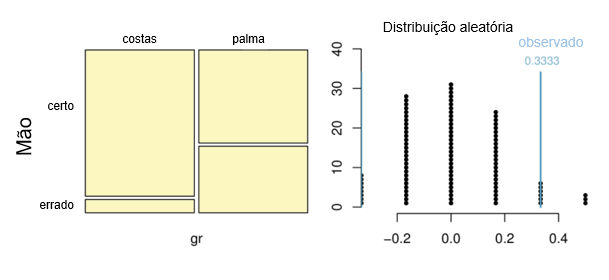
\includegraphics[width=0.8\textwidth,height=0.3\textheight]{6-6_small_two_props/palm_back_HT.png}

\end{frame}

%%%%%%%%%%%%%%%%%%%%%%%%%%%%%%%%%%%

\begin{frame}
\frametitle{Conclusão}
\justifying
\pq{Os resultados da simulação sugerem que as pessoas conhecem melhor o dorso das mãos do que a palma? \\
(Lembre-se: havia 33.3 \% mais acertos no grupo ddo dorso nos dados observados.)}

\begin{enumerate}[(a)]
\item Sim
\solnMult{Não}
\end{enumerate}
\justifying
p-valor = 0.09 $>$ 0.05, não rejeitar $H_0$. Os dados não fornecem evidências convincentes de que as pessoas conhecem melhor o dorso das mãos do que a palma das mãos.

\end{frame}

%%%%%%%%%%%%%%%%%%%%%%%%%%%%%%%%%%%%%


%%%%%%%%%%%%%%%%%%%%%%%%%%%%%%%%%%%%
% End document
%%%%%%%%%%%%%%%%%%%%%%%%%%%%%%%%%%%%

\end{document}